% !TeX spellcheck = ru_RU-Russian
% !TeX encoding = UTF-8 

\documentclass[14pt,a4paper]{extarticle}

\usepackage[russian]{babel}
\usepackage[utf8]{inputenc}
\usepackage{setspace} 
\usepackage[a4paper,
			left=30mm,
			right=10mm,
			top=20mm,
			bottom=20mm]{geometry}
\usepackage{amsmath}
\usepackage{amssymb}
\usepackage{amsthm}
\usepackage{graphicx} 
\usepackage{cite}
\usepackage{subfigure}
\usepackage{subcaption}
\usepackage{kprj} 
\usepackage{listings}
\usepackage{tabu}
\usepackage{courier}

\lstset{
	frame=single,
	basicstyle=\ttfamily,
	breaklines=true,
	tabsize=4
}

\VKR

\title{Инвариантные компакты и устойчивость положений равновесия в модели взаимодействия клеток иммунитета и мозговой опухоли}
\author{М.Д.~Кирдин}
\authorfull{Кирдин Матвей Дмитриевич}
\group{ФН12-81Б}
\faculty{Фундаментальные науки}
\chair{Математическое моделирование}
\chief{А.П.~Крищенко}
\inspector{М.А.~Велищанский}
\workyear{2024}
\facultyshort{ФН}
\chairshort{ФН12}
\chairhead{А.П.~Крищенко}

\onehalfspacing

\begin{document}
	\maketitle
	
	\begin{annotation}
	
	Расчетно-пояснительная записка 60 с., 13 рис., 22  источника.
	
	\MakeUppercase{функция Ляпунова; инвариантные компакты; злокачественные глиомы; аттрактор.}
	
	Данная работа описывает динамику развития злокачественных глиом с учетом их взаимодействия с иммунной системой при помощи системы обыкновенных дифференциальных уравнений. Предложенная математическая модель описывает взаимодействие клеток глиомы, макрофагов, активированных цитотоксичных Т-лимфоцитов(Т-киллеров), иммуноподавляющего фактора \textit{TGF-}$\beta$ и иммуностимулирующего фактора \textit{IFN-}$\gamma$. Динамика данной модели были исследована аналитически на предмет устойчивости с помощью методов локализации инвариантных компактов. Были найдены граничные положения равновесия, соответствующие отсутствию глиомы, а также было найдено компактное множество, содержащее аттрактор системы. При помощи численных методов было найдено и исследовано на предмет устойчивости и внутреннее положение равновесия при определенных значениях параметров.
	
	\end{annotation}
	
	\tableofcontents
	
	\begin{introduction}
	
	Глиомы --- тип опухолей головного или спинного мозга, развивающихся из глиальных клеток. Глиомы делятся на доброкачественные и злокачественные по степени агрессивности.  Доброкачественные опухоли растут медленно и не распространяются на другие органы, но они могут вызывать давление на мозг и нарушать его функции. Злокачественные глиомы быстро растут и могут распространяться на другие части мозга. В зависимости от структуры и мутаций, глиомы также разделяются на астроцитомы, олигодендроглиомы и глиобластомы \cite{glioma_classification}.
	
	Лечение глиом зависит от множества факторов, включая тип, размер и расположение опухоли, а также общее состояние здоровья пациента. Стандартные методы лечения включают хирургическое вмешательство, радиотерапию и химиотерапию. От 30\% до 40\% от всех мозговых опухолей \cite{glioma_overview} являются глиомами, поэтому последние годы значительные усилия были направлены на разработку иммунотерапии или оптимизации уже существующих методов, чтобы улучшить результаты лечения и качество жизни пациентов. Для этого необходимо исследование механизмов, лежащих в основе роста и распространения раковых клеток. Данная задача может быть решена путем составления и исследования математических моделей, описывающих динамику взаимодействия раковых и иммунных клеток в различных ситуациях. 
	
	Системы дифференциальных уравнений позволяют дать количественное представление многим биологическим процессам, протекающим во время заболевания \cite{abt_DEs}. Например, взаимодействие патогена и иммунной системы с учетом воздействия терапевтических белков\cite{Kasbawati et.al.}, реакция системы рак-иммунитет на химиотерапию\cite{W. L. Duan et.al.,Xiangdong Liu et.al.,L.G. de Pillis et.al., dePillis L.G. et.al.} или взаимодействие клеток иммунитета и раковых клеток с условием поражения ВИЧ т-хелперов\cite{F. A. Rihan et.al.}. В частности может быть предсказана динамику развития глиом в различных сценариях \cite{gliomae_scenarios}.
	
	Многие виды рака, включая опухоли головного и спинного мозга, подвергались системной иммунотерапии путем экзогенного введения иммунных клеток или иммунорегулирующих факторов с ограниченным успехом. Chakr-abarty и Hanson сформулировали задачу оптимального управления доставкой лекарств к опухоли мозга с целью минимизации плотности опухолевых клеток и снижения побочного действия лекарств с помощью метода конечных элементов Галеркина \cite{Chakrabarty et.al.}. Bandara и др. предложили математическую модель для рациональной разработки таргетных стратегий (in-silico) для эффективной транспортировки Паклитаксела, антимитотического препарата, через гематоэнцефалический барьер \cite{Bandera}. Kirkby и др. сформулировали модель глиобластомы, которая предсказывает эффекты эскалации дозы радиотерапии и воспроизводит чрезвычайно точные клинические данные \cite{Kirkby et.al.}. Schmitz и др. с помощью модели клеточного автомата опухоли мозга изучали гетерогенные опухоли, содержащие как чувствительные к лечению, так и резистентные к нему клетки. Авторы исследовали моноклональные опухоли, двухпоточные с резистентной субпопуляцией и многопоточные опухоли с индуцированной мутацией и смогли представить данные о времени выживания по каждому из этих примеров \cite{Schmitz et.al.}. Walker, Cook \cite{Walker et.al.} на макроскопической модели разработали систему доставки лекарств к опухолям мозга, где авторы предположили, что лекарство доставляется как в нормальную, так и в опухолевую ткань через сосудистую систему. Посредством диффузии и конвекции препараты проникают в ткани мозга через сосудистую сеть, переносятся через гематоэнцефалический барьер и интерстициальное пространство. Оценив влияние изменения параметров на доставку лекарств, они нашли оптимальный способ конвективной доставки лекарств в центр опухоли. Kronik и др. \cite{Kronik et.al.} рассмотрели интерактивную динамику цитотоксических Т-лимфоцитов, клеток опухоли мозга, основного комплекса гистосовместимости (MHC) класса-I и MHC класса-II, а также цитокинов \textit{TGF-}$\beta$ и \textit{IFN-}$\gamma$, где они использовали компьютерное моделирование для проверки модели и поиска предполагаемых сценариев лечения. Полученные ими результаты свидетельствуют о том, что глиобластома может быть уничтожена с помощью новых стратегий с интенсивной дозировкой или путем значительного стимулирования эндогенного иммунного ответа или инфузии Т-клеток, как показано в их математической модели.
	
	В данной работе была поставлена цель провести исследование модели, представленной в \cite{model} при помощи методов локализации инвариантных компактов \cite{invar_comp, invar_comp_localization}, исследование устойчивости положений равновесия системы при помощи построения функций Ляпунова.
	
	Нахождение инвариантных компактов позволит говорить об асимптотическом поведении траекторий системы, что на практике дает возможность судить о дальнейшем ходе заболевания по количествам клеток глиом, макрофагов, т-киллеров, белков \textit{TGF-}$\beta$, и гамма интерферонов.
	
	\end{introduction}
	
	\section{Локализация инвариантных компактов}
	\subsection{Постановка задачи}
	
	Рассмотрим следующую пятимерную систему с неотрицательными переменными $x=(x_1, x_2, x_3, x_4, x_5)$ и положительными параметрами:
	\begin{equation}
		\begin{cases}
			\begin{aligned}
				\dot{x}_1 &= r_1x_1\left(1-\dfrac{x_1}{c_1}\right)-\dfrac{1}{x_4+e_1}(\alpha_1x_2+\alpha_2x_3)\dfrac{x_1}{x_1+k_1},\\
				\dot{x}_2 &= r_2x_2\left(1-\dfrac{x_2}{c_2}\right)+\dfrac{x_5}{k_4+x_5}a_1\dfrac{1}{x_4+e_2}-\alpha_3\dfrac{x_1}{x_1+k_2}x_2,\\
				\dot{x}_3 &= a_2\dfrac{x_1}{k_5+x_4}-\mu_1x_3-\alpha_4\dfrac{x_1}{x_1+k_3}x_3,\\
				\dot{x}_4 &= s_1 + b_1x_1-\mu_2x_4,\\
				\dot{x}_5 &= b_2x_3-\mu_3x_5,
			\end{aligned}
		\end{cases}\label{eq:initial_system}
	\end{equation}
	где $t\ge0$ --- время;
	
	$x_1$ --- количество клеток глиомы; 
	
	$x_2$ --- количество макрофагов;
	
	$x_3$ --- количество т-киллеров;
	
	$x_4$ --- количество белков \textit{TGF-}$\beta$;
	
	$x_5$ --- количество $\gamma$-интерферонов. 
	
	Также из биологических соображений будем полагать, что начальные условия имеют следующий вид:
	\begin{equation}\label{eq:conds}
	x_1(0)\ge0,\,x_2(0)\ge0,\,x_3(0)\ge0,\,x_4(0)\ge0,\,x_5(0)\ge0.
	\end{equation}
	
	Введем следующие обозначения:
	\[\mathbb{R}^n_{+,0}=\{x=(x_1,\ldots,x_n)\in\mathbb{R}^n:\, x_i\ge0,\, i=\overline{1,n}\},\,\mathbb{R}_{+,0}=\{x\in\mathbb{R}:\, x\ge0\}.\]
	
	Для системы \ref{eq:initial_system} покажем, что множество $D=\mathbb{R}^{5}_{+,0} = \{x \ge 0\}$ положительно инвариантно, проведем исследование инвариантности пересечений множества $D$ с координатными плоскостями, а также систем, являющихся ограничениями \ref{eq:initial_system} на инвариантные координатные плоскости. Кроме того, найдем компактное множество, содержащее аттрактор системы.
	
	\subsection{Основные определения и теоремы}
	
	\begin{definition}
		Точка $p$ называется \textit{$\omega-$предельной точкой} траектории $x=x(t)$ в случае, если существует такая последовательность $\{t_n\}$, где $t_n\rightarrow+\infty$ при $n\rightarrow+\infty$, что $x(t_n)\rightarrow p$ при $n\rightarrow+\infty$. Множество всех предельных точек траектории $x=x(t)$ называется \textit{$\omega-$предельным множеством}.
	\end{definition}
	
	\begin{definition}
		Множество $M$ называется \textit{инвариантным} для непрерывной динамической системы $\dot{x} = F(x),\, x\in D\subset\mathbb{R}^n$, если 
		\[\forall{}x_0\in{}M\quad x(0)=x_0\implies{}x(t)\in{}M,\,\forall{}t\in\mathbb{R}.\]
		т.е. для любой точки $x_0\in M$ решение системы $x(t)$ с начальным условием $x(0)=x_0$ не выходит за пределы $M$ для любого $t\in\mathbb{R}$.
	\end{definition}
	
	\begin{definition}
		Множество $M$ называется \textit{положительно инвариантным} для непрерывной динамической системы $\dot{x} = F(x),\, x\in\mathbb{R}^n$, если 
		\[\forall{}x_0\in{}M\quad x(0)=x_0\implies{}x(t)\in{}M,\, t>0.\]
		т.е. для любой точки $x_0\in M$ решение системы $x(t)$ с начальным условием $x(0)=x_0$ не выходит за пределы $M$ при $t>0$.
	\end{definition}
	
	\begin{theorem}\cite[c.~20]{invar_comp}
		Все инвариантные множества динамической системы $\dot{x} = F(x),\, x\in D\subset\mathbb{R}^n,\, F\in C^1,$ содержащиеся в множестве $Q\subset D$, содержатся в \textit{локализирующем множестве}
		\[\Omega(\varphi,\, Q) = \left\{x\in Q:\, \varphi_{inf}(Q)\le \varphi(x) \le \varphi_{sup}(Q)\right\},\]
		где $\varphi(x)$ --- гладкая на множестве $D$ функция, называемая \textit{локализирующей функцией}, $\dot{\varphi}(x)$~---~производная $\varphi(x)$ в силу системы $\dot{x}=F(x)$,
		\[\varphi_{inf}(Q) = \inf\limits_{S(\varphi)\cap Q}\varphi(x),\,\,\varphi_{sup}(Q) = \sup\limits_{S(\varphi)\cap Q}\varphi(x),\]
		а $S(\varphi) = \left\{x\in\mathbb{R}^n:\, \dot{\varphi}(x)=0\right\}$ --- \textit{универсальное сечение} функции~$\varphi(x)$.
	\end{theorem}
	
	\begin{theorem}\cite[с.~84]{Arnold}\label{th:Arnold}
		Траектория динамической системы $\dot{x}=F(x)$ с начальным значением из любого компакта фазового пространства продолжается вперед(назад) либо неограниченно, либо до границы этого компакта.
	\end{theorem}
	
	\begin{theorem}\cite[c.~114]{Khalil}\label{th:Khalil}
		Если траектория $x=x(t)$ непрерывной динамической системы $\dot{x}=F(x),\, x\in D\subset\mathbb{R}^n$ ограничена и принадлежит $D$ при $t \ge 0$, то ее $\omega-$предельное множество --- непустой инвариантный компакт и $x(t)$ стремится к $\omega-$предельному множеству при $t\rightarrow+\infty$.
	\end{theorem}
	
	\subsection{Положительная инвариантность множества $D$}
	
	\begin{theorem}\textbf{(Коши)}
		Пусть функция $F(x, t)$ кусочно непрерывна по t и удовлетворяет неравенству
		\[\|F(x,t)-F(y,t)\|\le L\|x-y\|,\]
		где $L$ — постоянная, при любых x, y из $\varepsilon$-окрестности $O_{\varepsilon} = {x : \|x - x_0\| < \varepsilon}$ точки $x_0$ и любого $t \in [t_0,t_1]$. Тогда существует $\delta > 0$ для которого решение задачи Коши вида 
		\[\dot{x}=F(x,t),\, x(t_0)=x_0\in G,\, t\ge t_0,\]
		где $G$ -- область определения системы, существует и единственно при \linebreak$ t\in[t_0,t_0+\delta)$. 
	\end{theorem}
	
	\begin{affirmation}
		 Система \ref{eq:initial_system} с начальными условиями \ref{eq:conds} имеет, причем единственное, решение на области $D$. 
	\end{affirmation}
	\begin{proof}
		Правая часть системы --- непрерывно-дифференциируемая на множестве $D$ функция. Из этого следует, что она локально липшицева в каждой точке этого множества, т.е. для любой его точки справедлива теорема Коши. Таким образом, в каждой точке $D$ существует, причем единственное, решение задачи Коши.\qed
	\end{proof}
	
	\begin{theorem}
		Множество $D=\mathbb{R}^5_{+,0}$ является положительно инвариантным для системы~\ref{eq:initial_system}.
	\end{theorem}
	\begin{proof}
		Заметим, что граница множества $D$ --- множество точек с хотя бы одной нулевой координатой. Таким образом, достаточно показать, для траекторий системы, начинающихся на границе $D$, справедливо, что 
		\[x_i(t)\ge0,\, i=\overline{1,5},\, t\in[0,\,\varepsilon),\,\varepsilon>0.\]
		
		Рассмотрим следующий набор начальных условий:
		\begin{equation}\label{eq:conds_1}
			x_1(0)=0,\, x_2(0)\ge0,\, x_3(0)\ge0,\, x_4(0)\ge0,\, x_5(0)\ge0.
		\end{equation}
		Для каждого такого условия существует $\varepsilon_1>0$ такое, что существует, причем единственное, решение задачи Коши: 
		\begin{equation*}
			x_1=x_1(t),\, x_2=x_2(t),\, x_3=x_3(t),\, x_4=x_4(t),\, x_5=x_5(t),
		\end{equation*}
		где $t\in[0,\varepsilon_1)$, обращающее систему \ref{eq:initial_system} в тождество. Решение $x_1(t)\equiv0$ удовлетворяет начальному условию $x_1(0)=0$. При подстановке $x_1(t)\equiv0$ в \ref{eq:initial_system} первое уравнение становится тождеством, а сама система преобразуется к следующему виду:
		\begin{equation*}
			\begin{cases}
				\begin{aligned}
					\dot{x}_2(t) &= r_2x_2(t)\left(1-\dfrac{x_2(t)}{c_2}\right)+\dfrac{x_5(t)}{k_4+x_5(t)}a_1\dfrac{1}{x_4(t)+e_2},\\
					\dot{x}_3(t) &= -\mu_1x_3(t),\\
					\dot{x}_4(t) &= s_1 - \mu_2x_4(t),\\
					\dot{x}_5(t) &= b_2x_3(t)-\mu_3x_5(t).
				\end{aligned}
			\end{cases}
		\end{equation*} 
		Определив $x_2(t),\ldots,x_5(t)$ как решения системы с пониженным порядком с начальными условиями \ref{eq:conds_1}, из единственности решения задачи Коши имеем, что
		\begin{equation*}
		x_1\equiv0,\, x_2=x_2(t),\, x_3=x_3(t),\, x_4=x_4(t),\, x_5=x_5(t),\, t\in[0,\,\varepsilon_1),
		\end{equation*}
		является решением исходной системы с начальными условиями \ref{eq:conds_1}, лежащим на плоскости $x_1=0$ и не покидающим области $D$ через неё.
		
		Для каждого из начальных условий вида
		\begin{equation*}
			x_1(0)\ge0,\, x_2(0)\ge0,\, x_3(0)\ge0,\, x_4(0)=0,\, x_5(0)\ge0,
		\end{equation*}
		имеется $\varepsilon_2>0$ такое, что существует единственное решение задачи Коши на полуинтервале $t\in[0,\varepsilon_2)$, обращающее систему \ref{eq:initial_system} в тождество. В этом случае 
		\[\dot{x}_4(0)=s_1+b_1x_1(0)>0,\]
		т.е. 
		\[x_4(t)>0,\, t\in(0,\,\varepsilon_2)\]
		и траектории не выходят из $D$ через плоскость $x_4=0$.
		
		Рассмотрим случай, когда
		\begin{equation}\label{eq:conds_3}
			x_1(0)\ge0,\, x_2(0)\ge0,\, x_3(0)=0,\, x_4(0)\ge0,\, x_5(0)\ge0.
		\end{equation}
		Для каждого такого начального условия имеется $\varepsilon_3>0$ такое, что существует единственное решение задачи Коши на $t\in[0,\varepsilon_3)$ обращающее систему \ref{eq:initial_system} в тождество. Рассмотрим исходную систему при $t=0$:
		\begin{equation*}
			\begin{cases}
				\begin{aligned}
					\dot{x}_1(0) &= r_1x_1(0)\left(1-\dfrac{x_1(0)}{c_1}\right)-\dfrac{\alpha_1x_2(0)}{x_4(0)+e_1}\dfrac{x_1(0)}{x_1(0)+k_1},\\
					\dot{x}_2(0) &= r_2x_2(0)\left(1-\dfrac{x_2(0)}{c_2}\right)+\dfrac{x_5(0)}{k_4+x_5(0)}\dfrac{a_1}{x_4(0)+e_2}-\alpha_3\dfrac{x_1(0)}{x_1(0)+k_2}x_2(0),\\
					\dot{x}_3(0) &= a_2\dfrac{x_1(0)}{k_5+x_4(0)},\\
					\dot{x}_4(0) &= s_1 + b_1x_1(0)-\mu_2x_4(0),\\
					\dot{x}_5(0) &= -\mu_3x_5(0).
				\end{aligned}
			\end{cases}
		\end{equation*}
		Если $x_1(0)>0$, то и $\dot{x}_3(0)>0$, из чего $x_1(t)>0,\, t\in(0,\, \tilde{\varepsilon}_3),\,\tilde{\varepsilon}_3\le\varepsilon_3$ и траектория не выходит из $D$ через плоскость $x_3=0$. Если же $x_1(0)=0$, то при $t=0$ система примет вид:
		\begin{equation*}
			\begin{cases}
				\begin{aligned}
					\dot{x}_1(0) &= 0,\\
					\dot{x}_2(0) &= r_2x_2(0)\left(1-\dfrac{x_2(0)}{c_2}\right)+\dfrac{x_5(0)}{k_4+x_5(0)}a_1\dfrac{1}{x_4(0)+e_2},\\
					\dot{x}_3(0) &= 0,\\
					\dot{x}_4(0) &= s_1 + b_1x_1(0)-\mu_2x_4(0),\\
					\dot{x}_5(0) &= -\mu_3x_5(0).
				\end{aligned}
			\end{cases}
		\end{equation*}
		Тогда, аналогично случаю с границей $x_1=0$, $x_1(t)\equiv0$. При этом решение $x_3(t)\equiv0$ удовлетворяет начальному условию $x_3(0)=0$. Подставив $x_3(t)\equiv0$ совместно с $x_1(t)\equiv0$ в исходную систему получим следующий результат:
		\begin{equation*}
			\begin{cases}
				\begin{aligned}
					\dot{x}_2(t) &= r_2x_2(t)\left(1-\dfrac{x_2(t)}{c_2}\right)+\dfrac{x_5(t)}{k_4+x_5(t)}a_1\dfrac{1}{x_4(t)+e_2},\\
					\dot{x}_4(t) &= s_1-\mu_2x_4(t),\\
					\dot{x}_5(t) &= -\mu_3x_5(t).
				\end{aligned}
			\end{cases}
		\end{equation*}
		Если определить $x_2,\, x_4,\, x_5$ как решения системы с пониженным порядком на плоскости $x_1=x_3=0$ с начальными условиями \ref{eq:conds_3}, то из единственности решения следует, что
		\[x_1\equiv0,\, x_2=x_2(t),\, x_3\equiv0,\, x_4=x_4(t),\, x_5=x_5(t),\, t\in[0,\,\varepsilon_3),\]
		является решением исходной системы для которого выполняются \ref{eq:conds_3} при $x_1(0)=0$, лежащим на плоскости $x_1=x_3=0$ и не покидающим области~$D$ через границу $x_3=0$.
	
		В случае если 
		\begin{equation}\label{eq:conds_4}
			x_1(0)\ge0,\, x_2(0)\ge0,\, x_3(0)\ge0,\, x_4(0)\ge0,\, x_5(0)=0.
		\end{equation}
		Для каждого такого начального условия существует $\varepsilon_4>0$ такое, что существует единственное решение задачи Коши при $t\in[0,\varepsilon_4)$ обращающее систему \ref{eq:initial_system} в тождество. При $t=0$ исходная система примет вид:
		\begin{equation*}
			\begin{cases}
				\begin{aligned}
					\dot{x}_1(0) &= r_1x_1(0)\left(1-\dfrac{x_1(0)}{c_1}\right)-\dfrac{1}{x_4(0)+e_1}(\alpha_1x_2(0)+\alpha_2x_3(0))\dfrac{x_1(0)}{x_1(0)+k_1},\\
					\dot{x}_2(0) &= r_2x_2(0)\left(1-\dfrac{x_2(0)}{c_2}\right)-\alpha_3\dfrac{x_1(0)}{x_1(0)+k_2}x_2(0),\\
					\dot{x}_3(0) &= a_2\dfrac{x_1(0)}{k_5+x_4(0)}-\mu_1x_3(0)-\alpha_4\dfrac{x_1(0)}{x_1(0)+k_3}x_3(0),\\
					\dot{x}_4(0) &= s_1 + b_1x_1(0)-\mu_2x_4(0),\\
					\dot{x}_5(0) &= b_2x_3(0).
				\end{aligned}
			\end{cases}
		\end{equation*}
		В случае если $x_3(0)>0$ получим, что $\dot{x}_5(0)>0$, из чего 
		\[x_5(t)>0,\, t\in(0,\, \tilde{\varepsilon}_4),\,\tilde{\varepsilon}_4\le\varepsilon_4\]
		и траектория не выходит из $D$ через плоскость $x_5=0$. При $x_3(0)=0$, в свою очередь, система в начальный момент преобразуется к следующему виду:
		\begin{equation*}
			\begin{cases}
				\begin{aligned}
					\dot{x}_1(0) &= r_1x_1(0)\left(1-\dfrac{x_1(0)}{c_1}\right)-\dfrac{\alpha_1x_2(0)}{x_4(0)+e_1}\dfrac{x_1(0)}{x_1(0)+k_1},\\
					\dot{x}_2(0) &= r_2x_2(0)\left(1-\dfrac{x_2(0)}{c_2}\right)-\alpha_3\dfrac{x_1(0)}{x_1(0)+k_2}x_2(0),\\
					\dot{x}_3(0) &= a_2\dfrac{x_1(0)}{k_5+x_4(0)},\\
					\dot{x}_4(0) &= s_1 + b_1x_1(0)-\mu_2x_4(0),\\
					\dot{x}_5(0) &= 0.
				\end{aligned}
			\end{cases}
		\end{equation*} 
		Здесь при $x_1(0)>0$ имеем, что $\dot{x}_3(0)>0$, то есть
		\[\ddot{x}_5(0)=b_2\dot{x}_3(0)-\mu_3\dot{x}_5(0)=b_2\dot{x}_3(0)>0.\] 
		Из этого следует, что $x_5(t)>0,\, t\in(0,\, \tilde{\varepsilon}^\prime_4),\,\tilde{\varepsilon}^\prime_4\le\varepsilon_4$ и траектория не выходит из $D$ через плоскость $x_5=0$. При $x_1(0)=0$ система в начальный момент примет следующий вид:
		\begin{equation*}
			\begin{cases}
				\begin{aligned}
					\dot{x}_1(0) &= 0,\\
					\dot{x}_2(0) &= r_2x_2(0)\left(1-\dfrac{x_2(0)}{c_2}\right),\\
					\dot{x}_3(0) &= 0,\\ 
					\dot{x}_4(0) &= s_1-\mu_2x_4(0),\\
					\dot{x}_5(0) &= 0.
				\end{aligned}
			\end{cases}
		\end{equation*}
		Тогда решения $x_1(t)\equiv0,\, x_3(t)\equiv0,\, x_5(t)\equiv0$ удовлетворяет начальным условиям \ref{eq:conds_4}. При их подстановке в исходную систему получим, что:
		\begin{equation*}
			\begin{cases}
				\begin{aligned}
					\dot{x}_2(t) &= r_2x_2(t)\left(1-\dfrac{x_2(t)}{c_2}\right),\\
					\dot{x}_4(t) &= s_1-\mu_2x_4(t).\\
				\end{aligned}
			\end{cases}
		\end{equation*}
		Если определить $x_2$ и $x_4$ как решения системы с пониженным порядком на плоскости $x_1=x_3=x_5=0$ с начальными условиями \ref{eq:conds_4}, то из единственности решения следует, что
		\[x_1\equiv0,\, x_2=x_2(t),\, x_3\equiv0,\, x_4=x_4(t),\, x_5\equiv0,\, t\in[0,\,\varepsilon_4),\]
		является решением исходной системы с начальными условиями \ref{eq:conds_4}, где
		\[x_1(0)=0,\, x_3(0)=0,\, x_5(0)=0,\]
		которое лежит на плоскости $x_1=x_3=x_5=0$ и не покидает область $D$ через границу $x_5=0$.
		
		Рассмотрим случай, когда
		\begin{equation}\label{eq:conds_5}
			x_1(0)\ge0,\, x_2(0)=0,\, x_3(0)\ge0,\, x_4(0)\ge0,\, x_5(0)\ge0.
		\end{equation}
		Для каждого такого начального условия также существует $\varepsilon_5>0$ такое, что существует единственное решение задачи Коши на полуинтервале $t\in[0,\,\varepsilon_5)$ обращающее систему исходную систему в тождество. В начальный момент времени \ref{eq:initial_system} принимает вид: 
		\begin{equation*}
			\begin{cases}
				\begin{aligned}
					\dot{x}_1(0) &= r_1x_1(0)\left(1-\dfrac{x_1(0)}{c_1}\right)-\dfrac{\alpha_2x_3(0)}{x_4(0)+e_1}\dfrac{x_1(0)}{x_1(0)+k_1},\\
					\dot{x}_2(0) &= \dfrac{x_5(0)}{k_4+x_5(0)}a_1\dfrac{1}{x_4(0)+e_2},\\
					\dot{x}_3(0) &= a_2\dfrac{x_1(0)}{k_5+x_4(0)}-\mu_1x_3(0)-\alpha_4\dfrac{x_1(0)}{x_1(0)+k_3}x_3(0),\\
					\dot{x}_4(0) &= s_1 + b_1x_1(0)-\mu_2x_4(0),\\
					\dot{x}_5(0) &= b_2x_3(0)-\mu_3x_5(0).
				\end{aligned}
			\end{cases}
		\end{equation*} 
		В случае, если $x_5(0)>0$ получим, что $\dot{x}_2(0)>0$, из чего 
		\[x_2(t)>0,\, t\in(0,\, \tilde{\varepsilon}_5),\,\tilde{\varepsilon}_5\le\varepsilon_5\]
		и траектория не выходит из $D$ через плоскость $x_2=0$. При $x_5(0)=0$, в свою очередь, система преобразуется к следующему виду:
		\begin{equation*}
			\begin{cases}
				\begin{aligned}
					\dot{x}_1(0) &= r_1x_1(0)\left(1-\dfrac{x_1(0)}{c_1}\right)-\dfrac{\alpha_2x_3(0)}{x_4(0)+e_1}\dfrac{x_1(0)}{x_1(0)+k_1},\\
					\dot{x}_2(0) &= 0,\\
					\dot{x}_3(0) &= a_2\dfrac{x_1(0)}{k_5+x_4(0)}-\mu_1x_3(0)-\alpha_4\dfrac{x_1(0)}{x_1(0)+k_3}x_3(0),\\
					\dot{x}_4(0) &= s_1 + b_1x_1(0)-\mu_2x_4(0),\\
					\dot{x}_5(0) &= b_2x_3(0).
				\end{aligned}
			\end{cases}
		\end{equation*}  
		В случае, если $x_3(0)>0$ получим, что $\dot{x}_5(0)>0$, из чего 
		\[\ddot{x}_2(0) = a_1\dfrac{\dot{x}_5(0)}{k_4(x_4(0)+e_2)} > 0.\]
		Тогда $x_2(t)>0,\, t\in(0,\, \tilde{\varepsilon}^{\prime}_5),\,\tilde{\varepsilon}^{\prime}_5\le\varepsilon_5$ и траектория не выходит из $D$ через плоскость $x_2=0$. При $x_3(0)=0$ заметим, что $\ddot{x}_2(0)=0$ и система в начальный момент примет следующий вид:
		\begin{equation*}
			\begin{cases}
				\begin{aligned}
					\dot{x}_1(0) &= r_1x_1(0)\left(1-\dfrac{x_1(0)}{c_1}\right),\\
					\dot{x}_2(0) &= 0,\\
					\dot{x}_3(0) &= a_2\dfrac{x_1(0)}{k_5+x_4(0)},\\
					\dot{x}_4(0) &= s_1 + b_1x_1(0)-\mu_2x_4(0),\\
					\dot{x}_5(0) &= 0.
				\end{aligned}
			\end{cases}
		\end{equation*} 
		Здесь при $x_1(0)>0$ имеем, что $\dot{x}_3(0)>0,\,\ddot{x}_5(0)>0$, то есть 
		\[x_3(t)>0,\, t\in(0,\, \tilde{\varepsilon}^{\prime\prime}_5),\,\tilde{\varepsilon}^{\prime\prime}_5\le\varepsilon_5.\]
		Из этого следует, что
		\[\dddot{x}_2(0) = a_1\dfrac{\ddot{x}_5(0)}{k_4(x_4(0)+e_2)}>0.\]
		и тогда $x_2(t)>0,\, t\in(0,\, \tilde{\varepsilon}^{\prime\prime}_5),\,\tilde{\varepsilon}^{\prime\prime}_5\le\varepsilon_5$ и траектория не выходит из $D$ через плоскость $x_2=0$. При $x_1(0)=0$ система в начальный момент примет следующий вид:
		\begin{equation*}
			\begin{cases}
				\begin{aligned}
					\dot{x}_1(0) &= 0,\\
					\dot{x}_2(0) &= 0,\\
					\dot{x}_3(0) &= 0,\\
					\dot{x}_4(0) &= s_1 - \mu_2x_4(0),\\
					\dot{x}_5(0) &= 0.
				\end{aligned}
			\end{cases}
		\end{equation*}
		Тогда решения $x_1(t)\equiv0,\, x_2(t)\equiv0,\, x_3(t)\equiv0,\, x_5(t)\equiv0$ удовлетворяет начальным условиям \ref{eq:conds_5}. 
		При их подстановке в исходную систему получим, что:
		\begin{equation*}
			\begin{cases}
				\begin{aligned}
					\dot{x}_4(t) &= s_1-\mu_2x_4(t),\\
				\end{aligned}
			\end{cases}
		\end{equation*} 
		Тогда если определить $x_4$ как решение системы с пониженным порядком на плоскости $x_1=x_2=x_3=x_5=0$ с начальными условиями \ref{eq:conds_5}, то из единственности решения следует, что
		\[x_1\equiv0,\, x_2\equiv0,\, x_3\equiv0,\, x_4=x_4(t),\, x_5\equiv0,\, t\in[0,\,\varepsilon_5),\]
		является решением исходной системы с начальными условиями \ref{eq:conds_5}, где
		\[x_1(0)=0,\, x_2(0)=0,\, x_3(0)=0,\, x_5(0)=0,\]
		которое лежит на плоскости $x_1=x_2=x_3=x_5=0$ и не покидает область $D$ через границу $x_2=0$. Таким образом. траектории системы не пересекают ни одну из границ $x_i=0,\, i\in\overline{1,5}$.\qed
	\end{proof}
	
	Заметим, что из доказательства данной теоремы следует, что некоторые координатные плоскости положительно инвариантны относительно системы~\ref{eq:initial_system}. Для координатных плоскостей $x_i=0$ условие инвариантности -- выполнение равенств $\dot{x}_i=0$ для траекторий, начинающихся в них. Таким образом, плоскости  
	\begin{align*}
		x_1&=0;\\
		x_1&=0,\, x_3=0;\\
		x_1&=0,\, x_3=0,\, x_5=0,
	\end{align*}
	а также прямая $x_1=0,\, x_2=0,\, x_3=0,\, x_5=0$ являются инвариантными относительно исходной системы.  
	
	Рассмотрим плоскость $x_1=0$. Исходная система на этом множестве принимает вид:
	\begin{equation*}
		\begin{cases}
			\begin{aligned}
				\dot{x}_2 &= r_2x_2\left(1-\dfrac{x_2}{c_2}\right)+\dfrac{x_5}{k_4+x_5}a_1\dfrac{1}{x_4+e_2},\\
				\dot{x}_3 &= -\mu_1x_3,\\
				\dot{x}_4 &= s_1 - \mu_2x_4,\\
				\dot{x}_5 &= b_2x_3-\mu_3x_5.
			\end{aligned}
		\end{cases}
	\end{equation*}
	У преобразованной системы имеется два положения равновесия:
	\[P_1\left(0,0,\frac{s_1}{\mu_2},0\right),\, P_2\left(c_2,0,\frac{s_1}{\mu_2},0\right).\]
	
	Рассмотрим плоскость $x_1=0,\, x_3=0$. Исходная система на этом множестве принимает вид:
	\begin{equation*}
		\begin{cases}
			\begin{aligned}
				\dot{x}_2 &= r_2x_2\left(1-\dfrac{x_2}{c_2}\right)+\dfrac{x_5}{k_4+x_5}a_1\dfrac{1}{x_4+e_2},\\
				\dot{x}_4 &= s_1 -\mu_2x_4,\\
				\dot{x}_5 &= -\mu_3x_5.
			\end{aligned}
		\end{cases}
	\end{equation*}
	У данной системы также два положения равновесия:
	\[P_1\left(0,\frac{s_1}{\mu_2},0\right),\, P_2\left(c_2,\frac{s_1}{\mu_2},0\right).\]
	
	Рассмотрим плоскость $x_1=0,\, x_3=0,\, x_5=0$. Исходная система на этом множестве принимает вид:
	\begin{equation*}
		\begin{cases}
			\begin{aligned}
				\dot{x}_2 &= r_2x_2\left(1-\dfrac{x_2}{c_2}\right),\\
				\dot{x}_4 &= s_1 -\mu_2x_4,\\
			\end{aligned}
		\end{cases}
	\end{equation*}
	У преобразованной системы также два положения равновесия: $\left(0,\frac{s_1}{\mu_2}\right)$ и $\left(c_2,\frac{s_1}{\mu_2}\right)$.
	
	Рассмотрим прямую $x_1=0,\, x_2=0,\, x_3=0,\, x_5=0$. Исходная система на этом множестве принимает вид:
	\begin{equation*}
		\begin{aligned}
			\{\dot{x}_4 &= s_1 -\mu_2x_4,\\
		\end{aligned}
	\end{equation*}
	У данной системы единственное положение равновесия --- $x_4=\frac{s_1}{\mu_2}$.
	
	\subsection{Инвариантные множества внутри множества $D$}
	
	\begin{theorem}\label{th:inv_comp}
		Все компактные инвариантные множества системы (1) содержатся в положительно инвариантных множествах
		\begin{align*}
			K_1 &=\left\{0 \leqslant x_1 \leqslant \overline{x}_1 = c_1\right\}\cap D,\\[6pt]
			K_2 &=\left\{\dfrac{s_1}{\mu_2} = \underline{x}_4 \leqslant x_4 \leqslant \overline{x}_4 = \dfrac{s_1}{\mu_2} + b_1c_1\right\}\cap K_1,\\[6pt]
			K_3 &=\left\{0 \leqslant x_3 \leqslant \overline{x}_3 = \dfrac{a_2\overline{x}_1}{k_5+\underline{x}_4}\cdot\dfrac{\overline{x}_1+k_2}{\mu_1k_2}\right\}\cap K_2,\\[6pt]
			K_4 &=\left\{0 \leqslant x_5 \leqslant \overline{x}_5 = \dfrac{b_2\overline{x}_3}{\mu_3}\right\}\cap K_3,\\[6pt]
			K_5 &=\left\{0 \leqslant x_2 \leqslant \overline{x}_2 =  \dfrac{c_2}{2}+\sqrt{\dfrac{c_2^2}{4}+\dfrac{a_1\overline{x}_5}{k_4(\underline{x}_4+e_2)}}\right\}\cap K_4.
		\end{align*}
	\end{theorem}
	\begin{proof} 
		Пусть $\varphi_1(x)=x_1$. Тогда на области $D$:
		\[\dot{\varphi}_1(x)=r_1x_1\left(1-\dfrac{x_1}{c_1}\right)-\dfrac{1}{x_4+e_1}(\alpha_1x_2+\alpha_2x_3)\dfrac{x_1}{x_1+k_1}.\]
		Универсальное сечение на $D$ можно задать следующим образом:
		\[S(\varphi_1,\, D)=\left\{r_1x_1\left(1-\dfrac{x_1}{c_1}\right)-\dfrac{1}{x_4+e_1}(\alpha_1x_2+\alpha_2x_3)\dfrac{x_1}{x_1+k_1}=0\right\}\cap D.\]
		Преобразуем равенство, задающее это множество:
		\[S(\varphi_1,\, D)=\left\{x_1\left(r_1\left(1-\dfrac{x_1}{c_1}\right)-\dfrac{\alpha_1x_2+\alpha_2x_3}{(x_1+k_1)(x_4+e_1)}\right)=0\right\}\cap D.\]
		Тогда $x_1=0$ или $x_1=c_1\left(1-\dfrac{\alpha_1x_2+\alpha_2x_3}{r_1(x_1+k_1)(x_4+e_1)}\right) $. Таким образом, экстремальные значения $\varphi_1(x)$ на множестве $S(\varphi_1,\, D)$:
		\[\inf\limits_{x\in S(\varphi_1,\, D)} \varphi_1=0,\, \sup\limits_{x\in S(\varphi_1,\, D)} \varphi_1=c_1,\]
		из чего локализирующее множество $\Omega(\varphi_1,\, D)$ задается следующим образом:
		\[\Omega(\varphi_1,\, D)=\left\{0\leqslant x_1\leqslant c_1 = \overline{x}_1\right\}\cap D=K_1.\]
		
		Далее возьмем $\varphi_2(x)=x_4$. В таком случае универсальное сечение имеет вид:
		\[S(\varphi_2, K_1)=\left\{s_1 + b_1x_1-\mu_2x_4=0\right\}\cap K_1.\]
		На множестве $S(\varphi_2,\, K_1)$
		\[\inf\limits_{x\in S(\varphi_2,\, K_1)} \varphi_2=\dfrac{s_1}{\mu_2} = \underline{x}_4,\, \sup\limits_{x\in S(\varphi_2,\, K_1)} \varphi_2=\dfrac{s_1}{\mu_2}+\dfrac{b_1c_1}{\mu_2} = \overline{x}_4.\]
		Следовательно, локализирующее множество можно задать как 
		\[\Omega(\varphi_2,\, K_1)=\left\{\underline{x}_4 \leqslant x_4\leqslant \overline{x}_4\right\}\cap K_1=K_2.\]
		
		Пусть $\varphi_3(x)=x_3$. Универсальное сечение для данной функции:
		\[S(\varphi_3,\, K_2)=\left\{a_2\dfrac{x_1}{k_5+x_4}-\mu_1x_3-\alpha_4\dfrac{x_1}{x_1+k_3}x_3=0\right\}\cap K_2.\]
		Преобразовав выражение, задающее $S(\varphi_3,\, K_2)$, получим
		\[x_3=\dfrac{a_2x_1}{k_5+x_4}\cdot\dfrac{x_1+k_3}{\mu_1x_1+\mu_1k_3+\alpha_4x_1}.\]
		Тогда на множестве $S(\varphi_3,\, K_2)$
		\[\inf\limits_{x\in S(\varphi_3,\, K_2)} \varphi_3=0,\, \sup\limits_{x\in S(\varphi_3,\, K_2)} \varphi_3\leqslant \dfrac{a_2\overline{x}_1}{k_5+\underline{x}_4}\cdot\dfrac{\overline{x}_1+k_3}{\mu_1k_3}=\overline{x}_3.\]
		Таким образом, локализирующее множество:
		\[\Omega(\varphi_3,\, K_2) = (\{0\leqslant x_3 \leqslant \sup{x_3}\}\cap K_2) \subset (\{0 \leqslant x_3\leqslant \overline x_3\} \cap K_2) = K_3.\]
		
		Возьмем $\varphi_4(x)=x_5$. В таком случае универсальное сечение:
		\[S(\varphi_4,\, K_3)=\{\, b_2x_3-\mu_3x_5=0\}\cap K_3.\]
		На множестве $S(\varphi_4,\, K_3)$
		\[\inf\limits_{x\in S(\varphi_4,\, K_3)} \varphi_4=0,\, \sup\limits_{x\in S(\varphi_4,\, K_3)} \varphi_4=\dfrac{b_2\overline{x}_3}{\mu_3}=\overline{x}_5,\]
		поэтому 
		\[\Omega(\varphi_4,\, K_3) = \{0 \leqslant x_5 \leqslant \overline{x}_5\} \cap K_3 = K_4.\]
		
		Далее, пусть $\varphi_5(x)=x_2$. Тогда 
		\[S(\varphi_5,\, K_4)=\left\{r_2x_2\left(1-\dfrac{x_2}{c_2}\right)+\dfrac{x_5}{k_4+x_5}a_1\dfrac{1}{x_4+e_2}-\alpha_3\dfrac{x_1}{x_1+k_2}x_2=0\right\}\cap K_4.\]
		Рассмотрим равенство, задающее универсальное сечение $S_{\varphi_5}$. Заметим, что на множестве $S(\varphi_5,\, K_4)$:
		\begin{multline*}
			r_2x_2\left(1 - \dfrac{x_2}{c_2}\right) + \dfrac{x_5}{k_4+x_5}a_1\dfrac{1}{x_4+e_2} - \alpha_3\dfrac{x_1x_2}{x_1+k_2}\le\\
			\le r_2x_2\left(1-\dfrac{x_2}{c_2}\right) + \dfrac{a_1\overline{x}_5}{(\overline{x}_5+k_4)(\underline{x}_4+e_2)}.
		\end{multline*}
		Т.е.
		\[x_2^2-c_2x_2-\dfrac{a_1\overline{x}_5}{(\overline{x}_5+k_4)(\underline{x}_4+e_2)}\leqslant 0.\]
		Таким образом, 
		\[0 \leqslant x_2 \leqslant \dfrac{c_2}{2}+\sqrt{\dfrac{c_2^2}{4}+\dfrac{a_1\overline{x}_5}{(\overline{x}_5+k_4)(\underline{x}_4+e_2)}}=\overline{x}_2.\]
		Итого, локализирующее множество имеет следующий вид:
		\[\Omega(\varphi_5,\, K_4)=\{0\leqslant x_2 \leqslant \overline{x}_2\} \cap K_4 = K_5.\qed\]
	\end{proof}
	
	\begin{theorem}
		Множество $K_5$ является компактным и содержит аттрактор системы \ref{eq:initial_system}.
	\end{theorem}
	\begin{proof}
		Рассмотрим множество
		\[K_1(\tau_1) = \{0 \leqslant x_1 \leqslant c_1+\tau_1\}\cap D,\, \tau_1\geqslant0.\]
		Заметим, что на множестве $D\setminus K_1(\tau_1) = \{x_1>c_1+\tau_1\}$ производная локализирующей функции $\varphi_1$ в силу системы $\dot{\varphi}_1 < 0$. Действительно, на этом множестве 
		\[\dot{\varphi}_1 \leqslant r_1x_1\left(1-\dfrac{x_1}{c_1}\right) < -r_1(c_1+\tau_1)\dfrac{\tau_1}{c_1} \leqslant 0.\]
		Таким образом множества $K_1(\tau_1)$ положительно инвариантны. Далее будем говорить, что $c_1+\tau_1=\overline{\xi}_1(\tau_1)$.
		
		Рассмотрим множество 
		\[K_2(\tau_1,\,\tau_2,\, \tilde{\tau}_2)=\left\{\dfrac{s_1}{\mu_2}-\tilde{\tau}_2 \leqslant x_4 \leqslant \dfrac{s_1}{\mu_2} + \dfrac{b_1\overline{\xi}_1(\tau_1)}{\mu_2} + \tau_2\right\}\cap K_1(\tau_1),\,\tau_1,\,\tau_2,\,\tilde{\tau}_2 \geqslant 0.\]   
		На множестве $\left\{x_4 > \dfrac{s_1}{\mu_2} + \dfrac{b_1\overline{\xi}_1(\tau_1)}{\mu_2} + \tau_2\right\}\cap K_1(\tau_1)$
		\[\dot{\varphi_2} = s_1 + b_1x_1 - \mu_2x_4 < - \mu_2\tau_2 \leqslant 0.\]
		На множестве $\left\{x_4 < \dfrac{s_1}{\mu_2}-\tilde{\tau}_2\right\}\cap K_1(\tau_1)$
		\[\dot{\varphi_2} = s_1 + b_1x_1 - \mu_2x_4 > \mu_2\tilde{\tau}_2 \geqslant 0.\]
		Таким образом, множества $K_2(\tau_1,\,\tau_2,\,\tilde{\tau}_2)$ положительно инвариантны. Обозначим
		\begin{align*}
			\overline{\xi}_4(\tau_1,\,\tau_2) =&\, \dfrac{s_1}{\mu_2} + \dfrac{b_1\tilde{x}_1}{\mu_2} + \tau_2,\\
			\underline{\xi}_4(\tilde{\tau}_2) =&\, \dfrac{s_1}{\mu_2} - \tilde{\tau}_2.
		\end{align*}
		
		Пусть 
		\[K_3(\tau_1,\,\tau_2,\, \tilde{\tau}_2,\,\tau_3) = \left\{0 \leqslant x_3 \leqslant \dfrac{a_2\overline{\xi}_1(\tau_1)}{k_5+\underline{\xi}_4(\tilde{\tau}_2)}\cdot\dfrac{\overline{\xi}_1(\tau_1)+k_3}{\mu_1k_3}+\tau_3\right\}\cap K_2(\tau_1,\, \tau_2,\, \tilde{\tau}_2),\]
		где $\tau_1,\,\tau_2,\,\tilde{\tau}_2,\,\tau_3 \geqslant 0$. Тогда на множестве 
		\begin{multline*}
			K_2(\tau_1,\, \tilde{\tau}_2,\, \tau_2)\setminus K_3(\tau_1,\,\tau_2,\, \tilde{\tau}_2,\, \tau_3)=\\
			=\left\{x_3 > \dfrac{a_2\overline{\xi}_1(\tau_1)}{k_5+\underline{\xi}_4(\tilde{\tau}_2)}\cdot\dfrac{\overline{\xi}_1(\tau_1)+k_3}{\mu_1k_3}+\tau_3\right\}\cap K_2(\tau_1,\, \tau_2,\, \tilde{\tau}_2)
		\end{multline*}
		справедливо, что
		\begin{multline*}
			\dot{\varphi}_3 = a_2\dfrac{x_1}{k_5+x_4}-\mu_1x_3-\alpha_4\dfrac{x_1}{x_1+k_3}x_3 < a_2\dfrac{\overline{\xi}_1(\tau_1)}{k_5+\underline{\xi}_4(\tilde{\tau}_2)}-\\
			-\left(\mu_1+\alpha_4\dfrac{\overline{\xi}_1(\tau_1)}{\overline{\xi}_1(\tau_1)+k_3}\right) x_3 < a_2\dfrac{\overline{\xi}_1(\tau_1)}{k_5+\underline{\xi}_4(\tilde{\tau}_2)}-\dfrac{\mu_1k_3}{\overline{\xi}_1(\tau_1)+k_3} x_3 < -\dfrac{\mu_1k_2\tau_3}{\overline{\xi}_1(\tau_1)+k_2} \leqslant 0.
		\end{multline*}
		Таким образом, множества $K_3(\tau_1,\,\tau_2,\, \tilde{\tau}_2,\, \tau_3)$ положительно инвариантны. Далее будем считать, что
		\[\overline{\xi}_3(\tau_1,\,\tau_2,\, \tilde{\tau}_2,\, \tau_3) = \dfrac{a_2\overline{\xi}_1(\tau_1)}{k_5+\underline{\xi}_4(\tilde{\tau}_2)}\cdot\dfrac{\overline{\xi}_1(\tau_1)+k_2}{\mu_1k_2} + \tau_3.\]
		
		Положим, что 
		\[K_4(\tau_1,\,\tau_2,\, \tilde{\tau}_2,\, \tau_3,\,\tau_4) = \left\{0 \leqslant x_5 \leqslant \dfrac{b_2\overline{\xi}_3(\tau_1,\,\tau_2,\, \tilde{\tau}_2,\, \tau_3)}{\mu_3}+\tau_4\right\}\cap K_3(\tau_1,\,\tau_2,\, \tilde{\tau}_2,\, \tau_3),\]
		где $\tau_1,\,\tau_2,\, \tilde{\tau}_2,\, \tau_3,\,\tau_4 \geqslant 0$. На множестве 
		\begin{multline*}
			K_3(\tau_1,\,\tau_2,\, \tilde{\tau}_2,\, \tau_3)\setminus K_4(\tau_1,\,\tau_2,\,\tilde{\tau}_2,\,\tau_3,\,\tau_4) =\\
			=\left\{x_5 > \dfrac{b_2\overline{\xi}_3(\tau_1,\,\tau_2,\,\tilde{\tau}_2,\,\tau_3)}{\mu_3}+\tau_4\right\}\cap K_3(\tau_1,\,\tau_2,\, \tilde{\tau}_2,\, \tau_3)
		\end{multline*}
		справедливо, что
		\[\dot{\varphi}_4 = b_2x_3 - \mu_3x_5 < -\mu_3\tau_4 \leqslant 0,\]
		из чего множества $K_4(\tau_1,\,\tau_2,\,\tilde{\tau}_2,\,\tau_3,\,\tau_4)$ за положительно инвариантны. Обозначим
		\[\overline{\xi}_5(\tau_1,\,\tau_2,\,\tilde{\tau}_2,\,\tau_3,\,\tau_4) = \dfrac{b_2\overline{\xi}_3(\tau_1,\,\tau_2,\,\tilde{\tau}_2,\,\tau_3)}{\mu_3}+\tau_4.\]
		
		Рассмотрим множество 
		\begin{multline*}
			K_5(\tau_1,\,\tau_2,\,\tilde{\tau}_2,\,\tau_3,\,\tau_4,\,\tau_5) = \biggr\{0 \leqslant x_2 \leqslant \dfrac{c_2}{2}+\\
			+\sqrt{\dfrac{c_2^2}{4}+\dfrac{a_1\overline{\xi}_5(\tau_1,\,\tau_2,\,\tilde{\tau}_2,\,\tau_3,\,\tau_4)}{k_4(\underline{\xi}_4(\tilde{\tau}_2)+e_2)}}+\tau_5\biggr\}\cap K_4(\tau_1,\,\tau_2,\,\tilde{\tau}_2,\,\tau_3,\,\tau_4),
		\end{multline*}
		где $\tau_1,\,\tau_2,\,\tilde{\tau}_2,\,\tau_3,\,\tau_4,\,\tau_5 \geqslant 0$.
		Можно провести следующую оценку $\dot{\varphi}_2$:
		\[\dot{\varphi}_2 \leqslant r_2x_2\left(1-\dfrac{x_2}{c_2}\right)+\dfrac{a_1\overline{\xi}_5(\tau_1,\,\tau_2,\,\tilde{\tau}_2,\,\tau_3,\,\tau_4)}{(\overline{\xi}_5(\tau_1,\,\tau_2,\,\tilde{\tau}_2,\,\tau_3,\,\tau_4)+k_4)(\underline{\xi}_4(\tilde{\tau}_2)+e_2)}.\]
		Пусть
		\begin{align*}
			\overline{\xi}_2(\tau_1,\,\tau_2,\,\tilde{\tau}_2,\,\tau_3,\,\tau_4) = \dfrac{c_2}{2}+\sqrt{\dfrac{c_2^2}{4}+\dfrac{a_1\overline{\xi}_5(\tau_1,\,\tau_2,\,\tilde{\tau}_2,\,\tau_3,\,\tau_4)}{(\overline{\xi}_5(\tau_1,\,\tau_2,\,\tilde{\tau}_2,\,\tau_3,\,\tau_4)+k_4)(\underline{\xi}_4(\tilde{\tau}_2)+e_2)}},\\
			\underline{\xi}_2(\tau_1,\,\tau_2,\,\tilde{\tau}_2,\,\tau_3,\,\tau_4) = \dfrac{c_2}{2}-\sqrt{\dfrac{c_2^2}{4}+\dfrac{a_1\overline{\xi}_5(\tau_1,\,\tau_2,\,\tilde{\tau}_2,\,\tau_3,\,\tau_4)}{(\overline{\xi}_5(\tau_1,\,\tau_2,\,\tilde{\tau}_2,\,\tau_3,\,\tau_4)+k_4)(\underline{\xi}_4(\tilde{\tau}_2)+e_2)}}.
		\end{align*}
		В таком случае, на множестве 
		\begin{multline*}
			K_4(\tau_1,\,\tau_2,\,\tilde{\tau}_2,\,\tau_3,\,\tau_4)\setminus K_5(\tau_1,\,\tau_2,\,\tilde{\tau}_2,\,\tau_3,\,\tau_4,\,\tau_5) =\\
			=\left\{x_2 > \overline{\xi}_2(\tau_1,\,\tau_2,\,\tilde{\tau}_2,\,\tau_3,\,\tau_4)+\tau_5\right\}\cap K_4(\tau_1,\,\tau_2,\,\tilde{\tau}_2,\,\tau_3,\,\tau_4)
		\end{multline*}
		имеет место оценка
		\begin{multline*}
			\dot{\varphi}_2 \leqslant -(x_2 - \overline{\xi}_2(\tau_1,\,\tau_2,\,\tilde{\tau}_2,\,\tau_3,\,\tau_4))(x_2 - \underline{\xi}_2(\tau_1,\,\tau_2,\,\tilde{\tau}_2,\,\tau_3,\,\tau_4)) <\\
			< -2\tau_5\cdot\sqrt{\dfrac{c_2^2}{4}+\dfrac{a_1\overline{\xi}_5(\tau_1,\,\tau_2,\,\tilde{\tau}_2,\,\tau_3,\,\tau_4)}{(\overline{\xi}_5(\tau_1,\,\tau_2,\,\tilde{\tau}_2,\,\tau_3,\,\tau_4)+k_4)(\underline{\xi}_4(\tilde{\tau}_2)+e_2)}} \leqslant 0.
		\end{multline*}
		Следовательно, множества $K_5(\tau_1,\,\tau_2,\,\tilde{\tau}_2,\,\tau_3,\,\tau_4,\,\tau_5)$ положительно инвариантны. Также можно заметить, что множества $K_5(\tau_1,\,\tau_2,\,\tilde{\tau}_2,\,\tau_3,\,\tau_4,\,\tau_5)$ компактны при
		\[\tau_1,\,\tau_2,\,\tilde{\tau}_2,\,\tau_3,\,\tau_4,\,\tau_5 \geqslant 0.\]
		
		Покажем, что множество $K_5$ содержит аттрактор системы. Согласно теореме \thref{th:Arnold}, решение автономной системы вида $\dot{x}=F(x)$, где $F(x)$ --- гладкое векторное поле, с начальным значением из любого компакта продолжается вперед неограниченно, либо до границы этого компакта. Для любой траектории системы \ref{eq:initial_system} существует такой набор $\tau_i = \hat{\tau}_i$, что ее начальная точка будет содержаться в множестве 
		\[\hat{K}_5 = K_5(\hat\tau_1,\,\hat\tau_2,\,\hat{\tilde{\tau}}_2,\,\hat\tau_3,\,\hat\tau_4,\,\hat\tau_5).\]
		Т.к. компакт $\hat{K}_5$ положительно инвариантен и $\dot{\varphi}_i(x)<0$ на границе $\hat{K}_5$, то решения, начинающиеся в $\hat{K}_5\setminus K_5$, не будут достигать границы $\hat{K}_5$ и могут быть неограниченно продолжены. Тогда траектории, начинающиеся в $\hat{K}_5$ ограничены и принадлежат этому компакту при $t\ge0$. Из теоремы \thref{th:Khalil} следует, что предельные множества траекторий из $\hat{K}_5$ --- непустые инвариантные компакты. Согласно теореме \thref{th:inv_comp}, $K_5$ содержит все инвариантные компакты системы, т.е. $K_5$ также содержит предельные множества траекторий из $\hat{K}_5$. Т.к. для любой точки из $D$ можно подобрать $\tau_i$ такие, что соответствующий компакт $K_5(\tau_1,\,\tau_2,\,\tilde{\tau}_2,\,\tau_3,\,\tau_4,\,\tau_5)$ ее содержит, можно сделать вывод о том, что $K_5$ содержит предельные множества всех траекторий, начинающихся в $D$. Таким образом, $K_5$ --- положительно инвариантный компакт, содержащий аттрактор системы.\qed
		
	\end{proof}	
	
	\section{Исследование положений равновесия}
	\subsection{Метод выбора кандидата-функции Ляпунова для систем c\linebreak дробно-рациональными правыми частями}
	
	Рассмотрим следующий класс динамических систем:
	\[\dot{x}_i=F_i(x),\, x=(x_1,\ldots,x_n)\in D,\, i=\overline{1,n},\]
	где $D = \mathbb{R}^{n}_{+,0}$, правые части $F_i(x)$ --- дробно-рациональные функции (далее ДРФ) вида 
	\[F_i(x)=\dfrac{P_i(x)}{Q_i(x)},\]
	где $P_i(x)$ и $Q_i(x)$ --- многочлены $n$ переменных $x=(x_1,\ldots,x_n)$, степень $P_i(x)$ равна $m_i$ и $Q_i(x)$ не имеет корней в~$D$. В случае если функция $F_i(x)$ кратна $x_i$, она имеет следующий вид:
	\[F_i(x)=x_i\tilde{F}(x) = x_i\dfrac{\tilde{P}_i(x)}{Q_i(x)},\]
	где $\tilde{F}_i(x)$ --- ДРФ $n$ переменных $x=(x_1,\ldots,x_n)$ такая, что ее числитель $\tilde{P}_i(x)$ --- многочлен порядка $m_i-1$, а $Q_i(x)$ -- многочлен конечного порядка, не имеющий корней в~$D$.
	
	Для динамических систем данного вида в качестве кандидата на функцию Ляпунова для внутреннего положения равновесия $\hat{x}=(\hat{x}_1,\ldots,\hat{x}_n)\in D$ можно принять следующее выражение:
	\[V(x)=2\sum\limits_{i\in\sigma_1}\tilde{k}_i\left(x_i-\hat{x}_i-\hat{x}_i\ln\dfrac{x_i}{\hat{x}_i}\right) + \dfrac{1}{2}\sum\limits_{j\in\sigma_2}\tilde{k}_j\left(x_j-\hat{x}_j\right)^2,\]
	где $\sigma_1$ --- множество номеров функций $F_i(x)$ кратных $x_i$;
	
	$\sigma_2$ --- множество всех остальных номеров функций $F_i(x)$;
	
	$\tilde{k}_i$ --- положительные параметры. 
	
	Производная такой функции в силу системы представима в виде квадратичной формы:
	\[\dot{V}(x)=(x-\hat{x})^{T}H(x)(x-\hat{x}),\]
	где $H(x)$ -- симметричная функциональная матрица размера $n\times n$, координатными функциями которой являются дробно--рациональные функции. 
	
	На области $D$ для $V(x)$ выполняются следующие условия:
	\[V(x)>0,\, V(\hat{x})=0,\, \hat{x}\in D,\,x\in D\setminus\left\{\hat{x}\right\}.\]
	Действительно, квадратичные слагаемые неотрицательно определены на области $D$, а слагаемые вида
	\[x_i-\hat{x}_i-\hat{x}_i\ln\dfrac{x_i}{\hat{x}_i}\] 
	также неотрицательны в $D$. Производная $V(x)$ в силу системы имеет вид:
	\begin{multline*}
		\dot{V}(x)=\sum\limits_{i\in\sigma_1}\tilde{k}_i\left(1-\dfrac{\hat{x}_i}{x_i}\right)x_i\tilde{F}_i(x)+\sum\limits_{j\in\sigma_2}\tilde{k}_j(x_j-\hat{x}_j)F_j(x)=\\
		=\sum\limits_{i\in\sigma_1}\tilde{k}_i(x_i-\hat{x}_i)\tilde{F}_i(x)+\sum\limits_{j\in\sigma_2}\tilde{k}_j(x_j-\tilde{x}_j)F_j(x),
	\end{multline*}
	Разложим функции $P_i(x)$ по формуле Тейлора в точке $x=\hat{x}$ до порядка $m_i+1$. Поскольку $P_i(x)$~--- многочлен порядка $m_i$, остаточный член в данном разложении будет равен нулю. Заметим, что $\hat{x}$ --- положение равновесия, и поэтому $P_i(\hat{x})=0$, а
	\begin{equation}\label{eq:Taylor_poly}
		P_i(x) = \sum\limits_{|\tau|\le m_i}\dfrac{d^{\tau}{P}_i(\hat{x})}{\tau!}(x-\hat{x})^{\tau},
	\end{equation}
	где $\tau = (\tau_1,\ldots,\tau_n),\,\tau\in\mathbb{N}^{n}$ --- мультииндекс. Тогда разделив \ref{eq:Taylor_poly} на соответствующий многочлен $Q_i(x)$ получим, что функция $F_i(x)$ может быть представлена как
	\[F_i(x)=\sum\limits_{q\in\tilde{\sigma}_i}(x_p-\hat{x}_p)h_p(x),\]  
	где $h_p(x)$ -- ДРФ, $\tilde{\sigma}_i$ -- множество всех номеров $x_p,\, p\in\left\{1,\ldots,n\right\}$, входящих в $F_i(x)$. Из аналогичных соображений можно получить, что 
	\[
	\tilde{F}_i(x)=\sum\limits_{p\in\tilde{\sigma}^\prime_i}(x_p-\hat{x}_p)\tilde{h}_p(x),\]
	где $\tilde{h}_p(x)$ --- ДРФ, а $\tilde{\sigma}^\prime_i$ --- множество всех номеров $x_p,\, p\in\left\{1,\ldots,n\right\}$, входящих в $\tilde{F}_i(x)$.
	
	Тогда производная $V(x)$ в силу системы примет вид:
	\[\dot{V}(x)=\sum\limits_{i\in\sigma_1}\tilde{k}_i(x_i-\hat{x}_i)\sum\limits_{p\in\tilde{\sigma}^\prime_i}(x_p-\hat{x}_p)\tilde{h}_{p}(x)+\sum\limits_{j\in\sigma_2}\tilde{k}_j(x_j-\hat{x}_j)\sum\limits_{q\in\tilde{\sigma}_j}(x_q-\hat{x}_q)h_{q}(x).\]
	Сложив все слагаемые с повторяющимися множителями $(x_i-\hat{x}_i)(x_j-\hat{x}_i)$ и положив равными нулю коэффициенты при множителях отсутствующих в сумме, получим квадратичную форму с симметричной функциональной матрицей $H(x)$:
	\[\dot{V}(x)=(x-\hat{x})^{T}H(x)(x-\hat{x}).\]
	В случае если $H(x)$ отрицательно определена, можно сделать вывод о том, что внутреннее положение равновесия $\hat{x}$ асимптотически устойчиво. 

	\subsection{Положения равновесия на границе множества $D$}
	
	\begin{theorem}\textbf{(Ляпунова об устойчивости по первому приближению)}
		Пусть правая часть автономной системы $x = F(x),\quad x\in\mathbb{R}^n$, непрерывно дифференцируема в некоторой окрестности нулевого положения равновесия и $A = {\dfrac{\partial F(x)}{\partial x}\biggr\rvert}_{x=0}$. Тогда нулевое положение равновесия асимптотически устойчиво, если все корни характеристического уравнения матрицы $A$ имеют отрицательные действительные части, и неустойчиво, если у матрицы A есть корень характеристического уравнения с положительной действительной частью.
	\end{theorem}
	
	\begin{definition}
		Положение равновесия называется некритическим, если собственные значения матрицы его линейного приближения имеют ненулевые действительные части. Иначе ПР называется критическим. 
	\end{definition}
	
	\begin{theorem}\label{th:border_eqpoints}
		Система \ref{eq:initial_system} на границе области $D$ при положительных значениях параметров имеет положения равновесия $P_1\left(0,0,0,\frac{s_1}{\mu_2},0\right)$ и $P_2\left(0,c_2,0,\frac{s_1}{\mu_2},0\right)$. 
	\end{theorem}
	
	\begin{theorem}\label{th:border_stab}
		Положение равновесия $P_1\left(0,0,0,\frac{s_1}{\mu_2},0\right)$ является неустойчивым, а положение равновесия $P_2\left(0,c_2,0,\frac{s_1}{\mu_2},0\right)$ является асимптотически устойчивым при условии $k_1r_1s_1 + e_1k_1\mu_2r_1< \alpha_1c_2\mu_2$ и неустойчивым при условии $k_1r_1s_1 + e_1k_1\mu_2r_1>\alpha_1c_2\mu_2$. При $k_1r_1s_1 + e_1k_1\mu_2r_1 = \alpha_1c_2\mu_2$ необходимо дополнительное исследование.
	\end{theorem}
	\begin{proof}
		Заметим, что в некритических положениях равновесия, в отличие от критических, характеры устойчивости автономной системы и ее первого приближения в совпадают.
		Матрица Якоби исходной системы в точке $P_1$:
		\[\begin{pmatrix}
			r_{1} & 0 & 0 & 0 & 0\\ 
			0 & r_{2} & 0 & 0 & \frac{a_{1}}{k_{4}\,\left(e_{2}+\frac{s_{1}}{\mu _{2}}\right)}\\ 
			\frac{a_{2}}{k_{5}+\frac{s_{1}}{\mu _{2}}} & 0 & -\mu _{1} & 0 & 0\\ 
			b_{1} & 0 & 0 & -\mu _{2} & 0\\ 
			0 & 0 & b_{2} & 0 & -\mu _{3} 
		\end{pmatrix}.\]
		Набор ее собственных значений имеет вид
		\[\lambda_1=r_1,\quad \lambda_2=r_2,\quad \lambda_3=-\mu_1,\quad \lambda_4=-\mu_2,\quad \lambda_5=-\mu_3.\]
		Т.к. все параметры системы положительны, можно сделать вывод о том, что согласно теореме Ляпунова об устойчивости по первому приближению система \ref{eq:initial_system} неустойчива в ПР $P_1$.
		
		В точке $P_2$ матрица Якоби имеет вид:
		\[\begin{pmatrix}
			r_{1}-\frac{\alpha _{1}\,c_{2}}{k_{1}\,\left(e_{1}+\frac{s_{1}}{\mu _{2}}\right)} & 0 & 0 & 0 & 0\\ 
			-\frac{\alpha _{3}\,c_{2}}{k_{2}} & -r_{2} & 0 & 0 & \frac{a_{1}}{k_{4}\,\left(e_{2}+\frac{s_{1}}{\mu _{2}}\right)}\\ 
			\frac{a_{2}}{k_{5}+\frac{s_{1}}{\mu _{2}}} & 0 & -\mu _{1} & 0 & 0\\ 
			b_{1} & 0 & 0 & -\mu _{2} & 0\\ 
			0 & 0 & b_{2} & 0 & -\mu _{3}
		\end{pmatrix}.\]
		Ее набор собственных значений:
		\begin{multline*}
		\lambda_1=\dfrac{k_1r_1s_1 - \alpha_1c_2\mu_2 + e_1k_1\mu_2r_1}{k_1s_1 + e_1k_1\mu_2},\quad \lambda_2=-\mu_1,\\
		\lambda_3=-\mu_2,\quad \lambda_4=-\mu_3,\quad \lambda_5=-r_2.
		\end{multline*}
		Аналогично предыдущему случаю, из условия строгой положительности параметров системы следует, что в ПР $P_2$ система асимптотически устойчива при условии $k_1r_1s_1 + e_1k_1\mu_2r_1< \alpha_1c_2\mu_2$ и неустойчива при условии $k_1r_1s_1 + e_1k_1\mu_2r_1>\alpha_1c_2\mu_2$. Однако в случае когда $k_1r_1s_1 + e_1k_1\mu_2r_1=\alpha_1c_2\mu_2$ точка покоя $P_2$ является критической, т.е. теорема Ляпунова об устойчивости по первому приближению в этом случае не применима и необходимо дополнительное исследование.\qed
	\end{proof}
	
	\begin{theorem}\label{th:P2_stab}
		Положение $P_2\left(0,\, c_2,\,0,\,\dfrac{s_1}{\mu_2},\, 0\right)$ асимптотически устойчиво на инвариантной плоскости $G=\left\{x_1=x_3=x_5=0\right\}\cap D$. 
	\end{theorem}
	\begin{proof}
		На плоскости $G$ исходная система принимает следующий вид:
		\begin{equation}\label{eq:smol_sys}
			\begin{cases}
				\dot{x}_2=r_2x_2\left(1-\dfrac{x_2}{c_2}\right),\\
				\dot{x}_4=s_1-\mu_2x_4.
			\end{cases}
		\end{equation}
		Положение равновесия $P_2$ также будет являться положением равновесия для системы пониженного порядка \ref{eq:smol_sys} и эквивалентно точке $\tilde{P}_2\left(c_2,\, \dfrac{c_1}{\mu_2}\right)$ на плоскости $G$. Тогда рассмотрим следующую функцию Ляпунова:
		\[V(x_2,\, x_4)=2\tilde{k}_1\left(x_2-c_2-c_2\ln\dfrac{x_2}{c_2}\right)+\dfrac{1}{2}\tilde{k}_2\left(x_4-\dfrac{s_1}{\mu_2}\right)^2,\]
		где $\tilde{k}_1,\tilde{k}_2$ --- положительные числовые коэффициенты. Производная функции Ляпунова в силу системы таким образом:
		\[\dot{V}(x_2,\,x_4)=-(x_2-c_2)\tilde{k}_1\dfrac{r_2}{c_2}(x_2-c_2)-\left(x_4-\dfrac{s_1}{\mu_2}\right)\mu_2\tilde{k}_2\left(x_4-\dfrac{s_1}{\mu_2}\right).\]
		Ее можно представить как квадратичную форму следующего вида:
		\[\dot{V}(x_2,\, x_4)=\begin{pmatrix}
			x_2-c_2 & x_4-\dfrac{s_1}{\mu_2}
		\end{pmatrix}\begin{pmatrix}
			a_{11} & \dfrac{1}{2}a_{12}\\
			\dfrac{1}{2}a_{21} & a_{22}
		\end{pmatrix}\begin{pmatrix}
			x_2-c_2\\
			x_4-\dfrac{s_1}{\mu_2}
		\end{pmatrix},\]
		где $a_{11}=-\dfrac{r_2\tilde{k}_1}{c_2},\, a_{12}=a_{21}=0,\, a_{22}=-\mu_2\tilde{k}_2$. Пусть
		\[A=\begin{pmatrix}
			a_{11} & \dfrac{1}{2}a_{12}\\
			\dfrac{1}{2}a_{21} & a_{22}
		\end{pmatrix}=\begin{pmatrix}
			-\dfrac{r_2\tilde{k}_1}{c_2} & 0\\
			0 & -\mu_2\tilde{k}_2
		\end{pmatrix}\]
		Согласно критерию Сильвестра, если 
		\[a_{11}<0,\, \det A>0,\]
		то квадратичная форма, соответствующая $\dot{V}(x_2,\, x_4)$, отрицательно определена. Легко заметить, что 
		\begin{align*}
			a_{11} &= -\dfrac{r_2\tilde{k}_1}{c_2}<0,\\
			\det A &= a_{11}a_{22}-\dfrac{1}{4}a^2_{12} = \dfrac{r_2\mu_2\tilde{k}_1\tilde{k}_2}{c_2}>0
		\end{align*}
		при положительных значениях параметров. Таким образом, 
		\[V(x)>0,\, \dot{V}(x)<0,\, x\in G\setminus\left\{\tilde{P}_2\right\},\]
		из чего $\tilde{P}_2$ асимптотически устойчиво на $G$.\qed
	\end{proof}
	
	\subsection{Положения равновесия внутри области $D$}
	\begin{theorem}\label{th:inner_eqpoint}
		Если система \ref{eq:initial_system} при положительных значениях параметров имеет положения равновесия внутри области $D$, то их координаты являются нулями функции
		\[f(x_1)=r_2x_2\left(1-\dfrac{x_2}{c_2}\right)+\dfrac{x_5}{k_4+x_5}a_1\dfrac{1}{x_4+e_2}-\alpha_3\dfrac{x_1}{x_1+k_2}x_2,\]
		где $x_2,\ldots,x_5$ --- функции от $x_1$.
	\end{theorem}
	\begin{proof}
		В общем случае координаты внутренних положений равновесия удовлетворяют следующей системе уравнений:
		\begin{equation}\label{eq:equlibrium_points}
			\begin{cases}
				\begin{aligned}
					0 &= r_1x_1\left(1-\dfrac{x_1}{c_1}\right)-\dfrac{1}{x_4+e_1}(\alpha_1x_2+\alpha_2x_3)\dfrac{x_1}{x_1+k_1},\\
					0 &= r_2x_2\left(1-\dfrac{x_2}{c_2}\right)+\dfrac{x_5}{k_4+x_5}a_1\dfrac{1}{x_4+e_2}-\alpha_3\dfrac{x_1}{x_1+k_2}x_2,\\
					0 &= a_2\dfrac{x_1}{k_5+x_4}-\mu_1x_3-\alpha_4\dfrac{x_1}{x_1+k_3}x_3,\\
					0 &= s_1 + b_1x_1-\mu_2x_4,\\
					0 &= b_2x_3-\mu_3x_5.
				\end{aligned}
			\end{cases}
		\end{equation}
		Разрешив последние два уравнения системы \ref{eq:equlibrium_points} относительно $x_4$ и $x_5$, можно получить, что: 
		\[x_3=\dfrac{b_2}{\mu_3}x_5,\, x_4=\dfrac{b_1x_1+s_1}{\mu_2}.\]
		Разрешив третье уравнение системы \ref{eq:equlibrium_points} относительно $x_3$ получим следующее выражение:
		\[x_3 = a_2\dfrac{x_1}{k_5+x_4}\dfrac{x_1+k_3}{\alpha_4x_1+\mu_1(x_1+k_3)}.\]
		Первое уравнение системы \ref{eq:equlibrium_points} разрешимо относительно $x_2$, т.к. координаты внутренних положений равновесия строго положительны. Тогда
		\[x_2 = \dfrac{1}{\alpha_1}\left(r_1\left(1-\dfrac{x_1}{c_1}\right)(x_4+e_1)(x_1+k_1)-\alpha_2x_3\right).\]
		Таким образом, координаты внутренних положений равновесия системы \ref{eq:initial_system} задаются следующей системой соотношений:
		\begin{equation}\label{eq:P3_equations}
			\begin{cases}
				\begin{aligned}
					0 &= r_2x_2\left(1-\dfrac{x_2}{c_2}\right)+\dfrac{x_5}{k_4+x_5}a_1\dfrac{1}{x_4+e_2}-\alpha_3\dfrac{x_1}{x_1+k_2}x_2,\\
					x_2 &= \dfrac{1}{\alpha_1}\left(r_1\left(1-\dfrac{x_1}{c_1}\right)(x_4+e_1)(x_1+k_1)-\alpha_2x_3\right),\\
					x_3 &= a_2\dfrac{x_1}{k_5+x_4}\dfrac{x_1+k_3}{\alpha_4x_1+\mu_1(x_1+k_3)},\\
					x_4 &= \dfrac{b_1x_1+s_1}{\mu_2},\\
					x_5 &= \dfrac{b_2}{\mu_3}x_3.
				\end{aligned}
			\end{cases}
		\end{equation}
		Заметим, что подстановкой уравнений системы \ref{eq:P3_equations} друг в друга можно получить явные выражения координат $x_2,\ldots,x_5$ через $x_1$. Т.к. внутреннее положение равновесия лежит внутри области $D$, из второго уравнения системы \ref{eq:P3_equations} следует, что на координату $x_1$ точек покоя накладывается условие $0 < x_1 < c_1$. Тогда задача поиска внутреннего положения равновесия сводится к поиску нулей функции в правой части первого уравнения системы~\ref{eq:P3_equations}
		\[f(x_1)=r_2x_2\left(1-\dfrac{x_2}{c_2}\right)+\dfrac{x_5}{k_4+x_5}a_1\dfrac{1}{x_4+e_2}-\alpha_3\dfrac{x_1}{x_1+k_2}x_2,\]
		где $x_2,\ldots,x_5$ --- функции от $x_1$, на интервале $x\in\left(0,\, c_1\right)$.\qed
	\end{proof}
	
	\subsection{Численное моделирование}
	
	\begin{example}
		Рассмотрим систему \ref{eq:initial_system} при значениях параметров, данных в~\cite{model_params}. Вследствие того, что в источнике указан только диапазон значений параметра $a_2$, положим, что $a_2=0.25$ (полный набор параметров указан в Приложении A). 
		
		Согласно теореме \thref{th:border_eqpoints}, система имеет граничные положения равновесия
		\[P_1\left(0,\,0,\,0,\,9134.92,\,0\right),\, P_2\left(0,\,1000000,\,0,\,9134.92,\,0\right).\]
		Согласно теореме~\thref{th:border_stab}, положения равновесия $P_1$ и $P_2$ неустойчивы в $D$, однако стоит отметить, что, согласно теореме~\thref{th:P2_stab}, положение равновесия $P_2$ является асимптотически устойчивым на плоскости $x_1=x_3=x_5=0$. 
		
		В результате численного поиска нулей $f(x_1)$ было получено, что система имеет единственное внутреннее положение равновесия:
		\[P_3\left(875419,\,943092,\,151.6804,\,9135.65,\,0.15168\right).\]
		Проведем численное исследование устойчивости внутреннего положения равновесия и динамики траекторий. Матрица Якоби системы с заданными параметрами в точке $P_3$: 
		\[\begin{pmatrix}
			-0.009635&-0.000071&-0.000014& \phantom{-}0.003766&0\\
			-0.003638&-0.309228& 0       & 0.      & 0\\
			\phantom{-}0.000014& 0   &    -0.129571&-0.001766& 0\\
			0       & 0     &   0     &  -6.933988& 0\\
			0       & 0&\phantom{-}0.000102& 0   &   -0.102000 
		\end{pmatrix}.\]
		Спектр данной матрицы имеет следующий вид:
		\begin{multline*}
			\lambda_1=-6.93399,\,\, \lambda_2=-0.309229,\\
			\lambda_3=-0.129571,\,\, \lambda_4=-0.102,\,\, \lambda_5=-0.009634.
		\end{multline*}
		Все собственные значения являются отрицательными действительными числами, т.е. положение равновесия $P_3$ асимптотически устойчиво.
		
		Естественный интерес представит динамика траектории системы, начинающейся в точке $\left(1,\,0,\,0,\,0,\,0\right)$, представляющей собой начало процесса развития глиомы у человека при условии отсутствия иммунотерапии. На \figref{fig:in_D} дано графическое представление динамики развития болезни в течение первых 3000 дней. Можно заметить, что популяция раковых клеток при $t=1500$~дням испытывает резкий скачок после чего останавливается на численности, соответствующей положению равновесия. Популяции макрофагов и клеток т-киллеров также испытывают скачки роста, после чего останавливаются на значениях, соответствующих внутреннему положению равновесия. Стоит заметить, что при $t=150$ дням популяция макрофагов стремится к максимально возможному значению. Иммуноподавляющий фактор $TGF-\beta$ достигает значений, близких внутреннему положению равновесия при $t=160$ дн, тем самым затрудняя рост популяций клеток иммунитета.

		\begin{figure}[h]
			\centering
			\subfigure[]{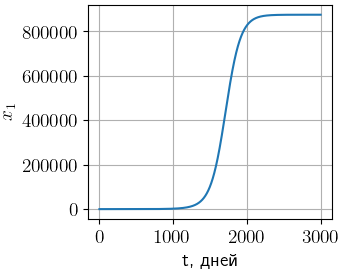
\includegraphics[width=0.35\textwidth]{media/Figure_1.png}} 
			\subfigure[]{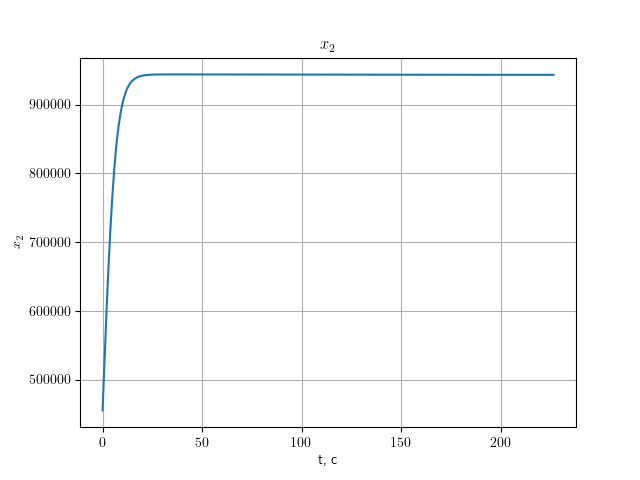
\includegraphics[width=0.35\textwidth]{media/Figure_2.png}}\\
			\subfigure[]{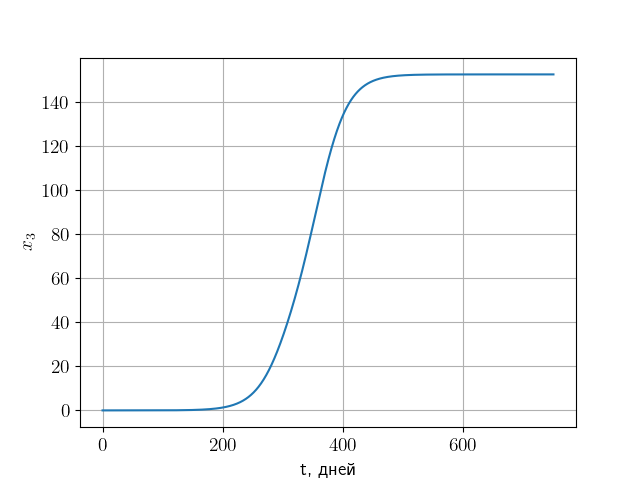
\includegraphics[width=0.32\textwidth]{media/Figure_3.png}}
			\subfigure[]{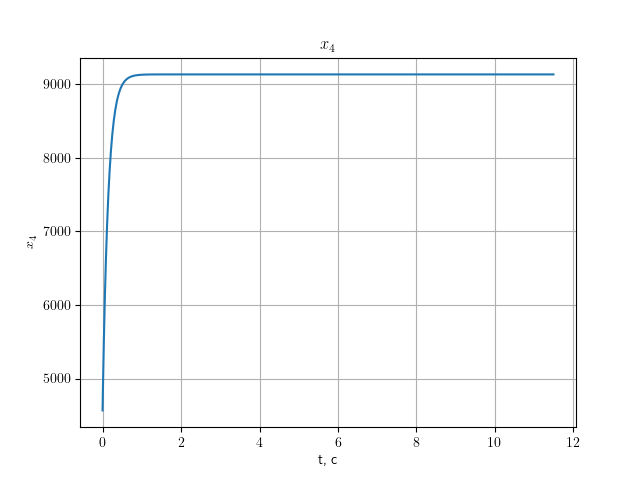
\includegraphics[width=0.32\textwidth]{media/Figure_4.png}}
			\subfigure[]{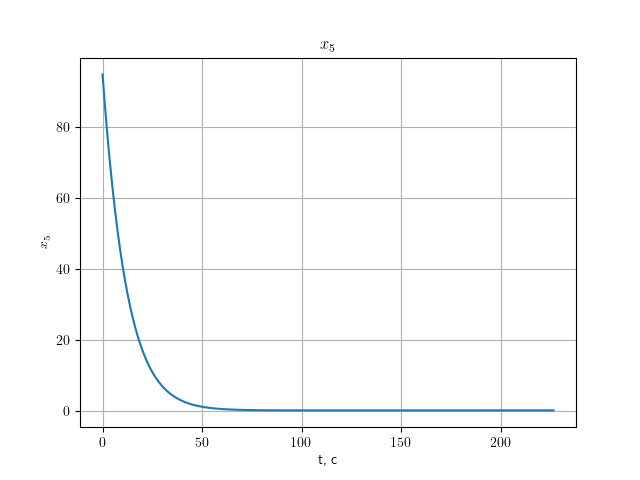
\includegraphics[width=0.32\textwidth]{media/Figure_5.png}}
			\caption{Переходные процессы системы для каждой координаты}
			\label{fig:in_D}
		\end{figure}
		\begin{figure}[h]
			\centering
			\subfigure[]{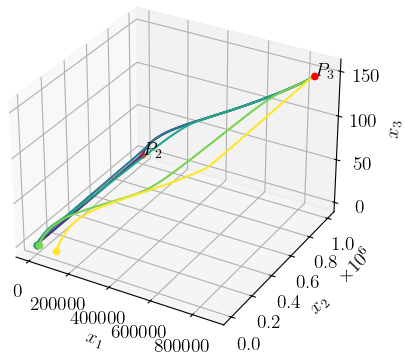
\includegraphics[width=0.33\textwidth]{media/Figure_8.png}} 
			\subfigure[]{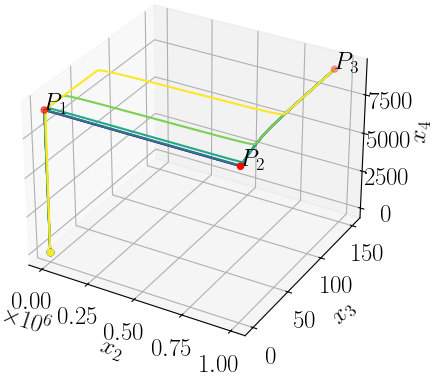
\includegraphics[width=0.32\textwidth]{media/Figure_9.png}}
			\subfigure[]{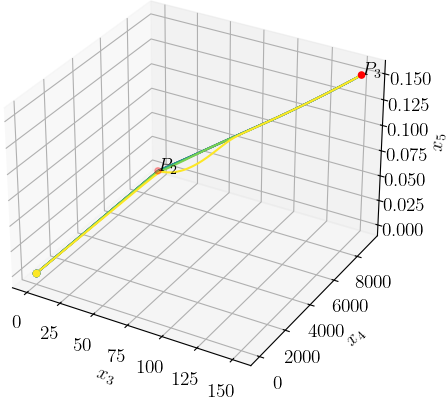
\includegraphics[width=0.33\textwidth]{media/Figure_10.png}}
			\caption{Переходные процессы системы для различных троек координат для шести вариантов значения $x_1$}
			\label{fig:in_D_3d}
		\end{figure}
		
		На \figref{fig:in_D_3d} показаны переходные процессы в различных тройках координат для начальных точек, соответствующих случаям, когда в исходном состоянии $x_1=1$, $x_1=10$, $x_1=100$, $x_1=1000$, $x_1=10000$ и $x_1=100000$. Из рисунка видно, что траектории изначально стремятся к положению равновесия $P_2$, соответствующему здоровому состоянию у пациента, после чего стремится к ПР $P_3$. Также на \figref{fig:x1_transitions} отдельно приведены переходные процессы для координаты $x_1$ с аналогичными начальными точками.
	
		\begin{figure}[h]
			\centering
			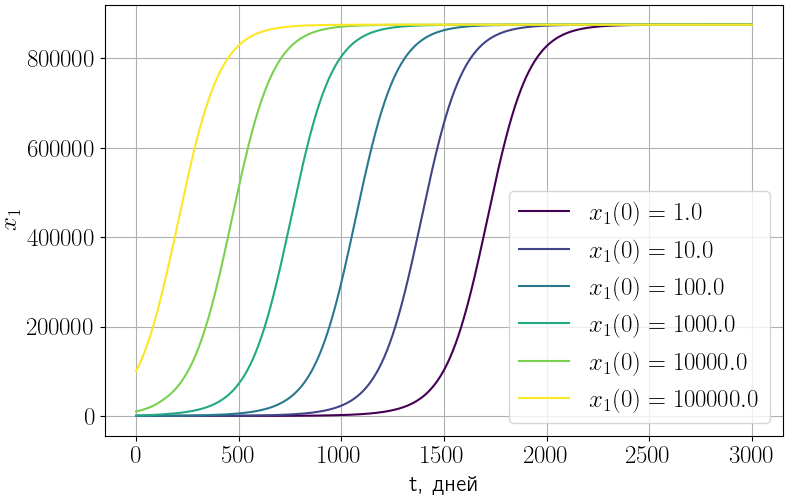
\includegraphics[width=0.90\textwidth]{media/Figure_12.png}
			\caption{Переходные процессы системы для различных начальных значений~$x_1$}
			\label{fig:x1_transitions}
		\end{figure}
		\begin{figure}[h]
			\centering
			\subfigure[]{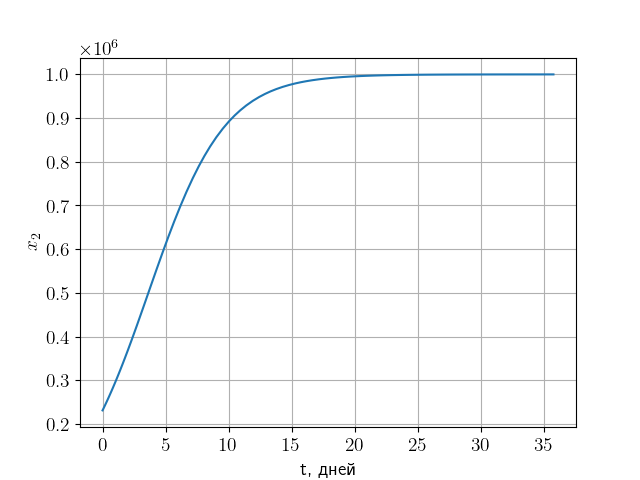
\includegraphics[width=0.40\textwidth]{media/Figure_6.png}} 
			\subfigure[]{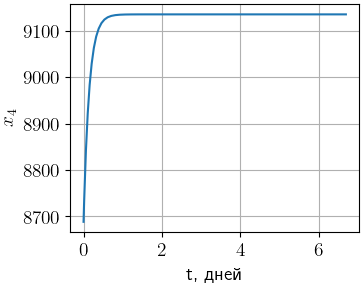
\includegraphics[width=0.40\textwidth]{media/Figure_7.png}}\\
			\caption{Переходные процессы системы при выборе начальной точки на плоскости $x_1=x_3=x_5=0$}
			\label{fig:on_D_border}
		\end{figure}
		
		Проведем аналогичное моделирование для случайной траектории на плоскости $x_1=x_3=x_5=0$. Из \figref{fig:on_D_border} можно делать вывод о том, что траектория приходит к положению равновесия $P_2$ за $t=35$ дней. Заметим, что в данном случае количество иммуноподавляющего фактора $TGF-\beta$ испытывает резкий скачок в результате которого достигает значений близких положению равновесия при $t=1$ дн. 
		
		\begin{figure}[h]
			\centering
			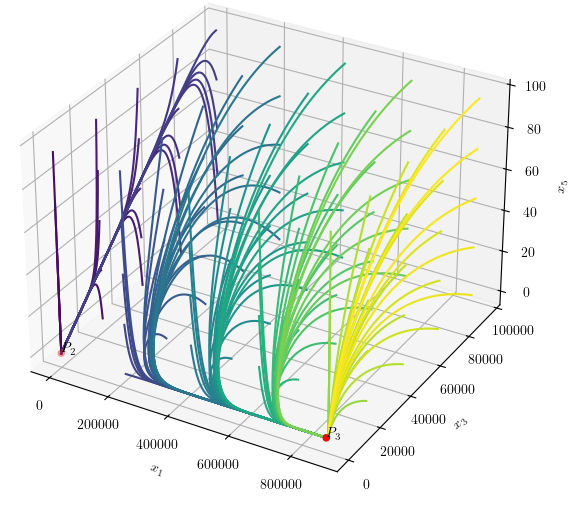
\includegraphics[width=0.60\textwidth]{media/Figure_11.png}
			\caption{Траектории системы в координатах $x_1,\, x_3,\, x_5$}
			\label{fig:model_K5}
		\end{figure}	
		
		На \figref{fig:model_K5} было проведено моделирование траекторий системы внутри множества $K_5$. Это показывает типичный ход траекторий системы внутри локализирующего множества. Видно, что траектории, начинающиеся в инвариантной плоскости $x_1=0$, остаются на ней. При этом траектории, начинающиеся вне нее стремятся к внутреннему положению равновесия.
	\end{example}
	
	\begin{example}
		В примере 1 был рассмотрен набор параметров при котором положение равновесия $P_2$ является неустойчивым в $D$. Рассмотрим обратный случай: выберем набор параметров при которых $P_2$ асимптотически устойчиво в~$D$. Согласно теореме~\thref{th:border_stab}, $P_2$ асимптотически устойчиво в $D$ в случае если
		\[k_1r_1s_1 + e_1k_1\mu_2r_1 < \alpha_1c_2\mu_2.\]
		Таким образом, если выбрать 
		\[r_1 < \dfrac{\alpha_1c_2\mu_2}{k_1s_1 + e_1k_1\mu_2}.\]
		Сохранив значения всех параметров из примера 1 кроме $r_1$, получим, что $r_1 < 0.002903$. Поэтому положим, что $r_1=0.002$.
		
		Из соображений, аналогичных изложенным в примере 1, можно получить, что при таком наборе параметров система имеет два граничных положения равновесия $P_1\left(0,\,0,\,0,\,9134.92,\,0\right)$ и $P_2\left(0,\,1000000,\,0,\,9134.92,\,0\right)$.
		Заметим, что в то время как $P_1$ остается неустойчивым, $P_2$, в силу выбора параметра~$r_1$, является асимптотически устойчивым в $D$. Также, согласно теореме~\thref{th:P2_stab}, $P_2$ асимптотически устойчиво на плоскости $x_1=x_3=x_5=0$. 
		
		\begin{figure}[h]
			\centering 
			\subfigure[]{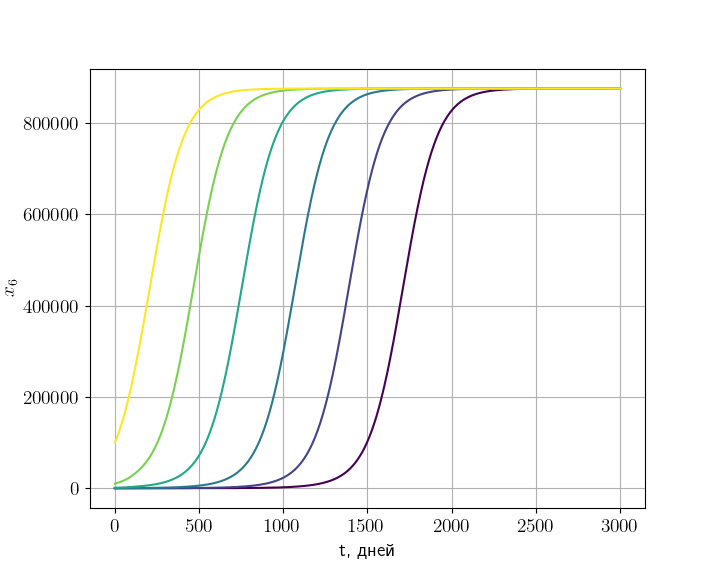
\includegraphics[width=0.90\textwidth]{media/Figure_13.png}}
			\caption{Переходные процессы системы с новыми параметрами для различных начальных значений~$x_1$}
			\label{fig:x1_transitions_new}
		\end{figure}
		
		Система также имеет единственное внутреннее положение равновесия 
		\[P_3\left(882650,\,0.000001,\,152.606,\,9135.65,\,0.152606\right).\]
		Матрица Якоби системы с новыми параметрами в точке $P_3$: 
		\[\begin{pmatrix}
			-0.00196&  -0.000076 &-0.000006&  0    &    0\\
			 0     &   \phantom{-}0.311876&  0     &   0    &    0\\
			 \phantom{-}0.000014&  0     &  -0.129852& -0.00178 &  0\\
			 0   &     0     &   0    &   -6.933988 & 0\\
			 0    &    0   &     \phantom{-}0.000102 & 0    &   -0.102\\
		\end{pmatrix}.\]
		Спектр данной матрицы имеет следующий вид:
		\begin{multline*}
			\lambda_1=-6.93399,\,\, \lambda_2=-0.129852,\\
			\lambda_3=-0.102,\,\, \lambda_4=-0.00196,\,\, \lambda_5=0.311876.
		\end{multline*}
		Собственное значение $\lambda_5$ является положительным действительным числом, следовательно, положение равновесия $P_3$ является неустойчивым. 
		
		Рассмотрим поведение траекторий в данном случае. В результате численного моделирования решений системы с начальными условиями вида 
		\[x_1(0)=x_{1,0},\, x_2(0)=0,\, x_3(0)=0,\, x_4(0)=0,\, x_5(0)=0,\, x_{1,0}\in\mathbb{R}_{+},\]
		было выяснено, что траектории стремятся к положению равновесия $P_2$ при $x_1 < 9273.02$, в противном случае --- к положению равновесия $P_3$(см. \figref{fig:x1_transitions_new}). 
		На \figref{fig:model_K5_new} было проведено моделирование траекторий системы внутри множества $K_5$. Это показывает типичный ход траекторий системы внутри локализирующего множества. Видно, что траектории, стремятся к положению равновесия $P_3$ только при $x_1>9273.02$.
		
		\begin{figure}[h]
			\centering
			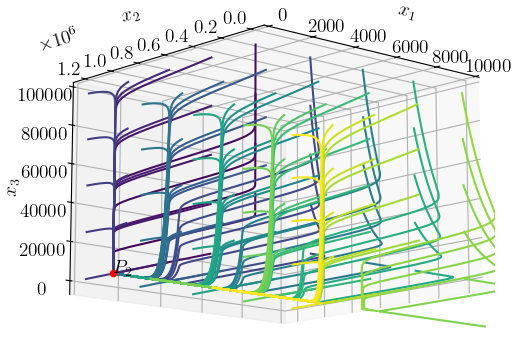
\includegraphics[width=0.60\textwidth]{media/Figure_16.png}
			\caption{Траектории системы в координатах $x_1,\, x_2,\, x_3$}
			\label{fig:model_K5_new}
		\end{figure}
	\end{example}
	
	\begin{conclusion}
	Математическое моделирование в онкологии играет важную роль, поскольку общие знания о причинах возникновения, механизме роста, методах устранения и лечения различных типов опухолей до сих пор остаются загадкой. Оно помогает ученым и врачам понять сложные процессы, происходящие в организме при развитии раковых заболеваний. Модель, рассмотренная в данной работе, позволяет оценить динамику взаимодействия между глиомой и иммунной системой.
	
	Было показано, что траектории системы начинающиеся в $D$ остаются в этом множестве. Это исключает нефизиологичные сценарии, при которых популяции клеток становятся отрицательными. Также было найдено компактное множество, содержащее аттрактор, что позволяет судить о ходе заболевания в долгосрочной перспективе.
	
	Было найдено два положения равновесия на границе множества. Они соответствуют сценариям, когда раковые клетки в начале отсутствуют и также не появляются новые, что может быть интерпретировано как здоровое состояние организма. Зная значения параметров системы возможно судить о наличии и устойчивости или неустойчивости внутреннего положения равновесия. При значениях параметров данных в \cite{model_params} внутренняя точка покоя существует и является асимптотически устойчивой. Это говорит о том, что иммунотерапия в данном случае не дает возможности полностью излечить заболевание. 
	
	Данные результаты могут быть использованы для оценки эффективности методов иммунотерапии, разработки новых, более эффективных терапий, а также для создания более точных математических моделей, которые учитывают больше переменных и могут предоставить еще более глубокое понимание взаимодействия между опухолью и иммунной системой. Такие модели могут включать различные типы иммунных клеток, учитывать пространственное распределение клеток опухоли и включать эффекты насыщения, которые могут влиять на реакцию иммунной системы.
	\end{conclusion}
	
	\def\bibindent{-0.8em}
	\begin{thebibliography}{\kern\bibindent} \makeatletter \let\old@biblabel\@biblabel \def\@biblabel#1{\hspace{12.5 mm}\old@biblabel{#1}\kern\bibindent} \let\old@bibitem\bibitem \def\bibitem#1{\old@bibitem{#1}\leavevmode\kern-\bibindent} \makeatother
		
		\bibitem{glioma_classification}
		Byun YH, Park CK. Classification and Diagnosis of Adult Glioma: A Scoping Review. Brain Neurorehabil. 2022 Nov 22;15(3):e23. doi: 10.12786/bn.2022.15.e23. PMID: 36742083; PMCID: PMC9833487.
		\bibitem{glioma_overview}
		Zeng T, Cui D, Gao L. Glioma: an overview of current classifications, characteristics, molecular biology and target therapies. Front Biosci (Landmark Ed). 2015 Jun 1;20(7):1104-15. doi: 10.2741/4362. PMID: 25961548.
		\bibitem{abt_DEs}
		S. Bunimovich-Mendrazitsky, J. C. Gluckman and J. Chaskalovic, J. Theor. Biol. 277,27 (2011).
		\bibitem{Kasbawati et.al.}
		Kasbawati, Yuliana Jao, Nur Erawaty. Dynamic study of the pathogen-immune system interaction with natural delaying effects and protein therapy[J]. AIMS Mathematics, 2022, 7(5): 7471-7488. doi: 10.3934/math.2022419
		\bibitem{W. L. Duan et.al.}
		W. L. Duan, H. Fang, C. Zeng, The stability analysis of tumor-immune responses to chemotherapy system with gaussian white noises. Chaos, Soliton. Fract., 127 (2019), 96–102. https://doi.org/10.1016/j.chaos.2019.06.030. doi: 10.1016/j.chaos.2019.06.030 
		\bibitem{Xiangdong Liu et.al.}
		Xiangdong Liu, Qingze Li, Jianxin Pan, A deterministic and stochastic model for the system dynamics of tumor–immune responses to chemotherapy, Physica A: Statistical Mechanics and its Applications, Volume 500, 2018, pp. 162-176, ISSN 0378-4371, https://doi.org/10.1016/j.physa.2018.02.118.
		\bibitem{L.G. de Pillis et.al.}
		L.G. de Pillis, W. Gu, K.R. Fister, T. Head, K. Maples, A. Murugan, T. Neal, K. Yoshida, Chemotherapy for tumors: An analysis of the dynamics and a study of quadratic and linear optimal controls, Mathematical Biosciences, Volume 209, Issue 1, 2007, pp. 292-315, ISSN 0025-5564, https://doi.org/10.1016/j.mbs.2006.05.003.
		\bibitem{dePillis L.G. et.al.}
		dePillis, L.G., Eladdadi, A. \& Radunskaya, A.E. Modeling cancer-immune responses to therapy. J Pharmacokinet Pharmacodyn 41, 461–478 (2014). https://doi.org/10.1007/s10928-014-9386-9
		\bibitem{F. A. Rihan et.al.}
		F. A. Rihan, D. H. A. Rahman, Delay differential model for tumour-immune dynamics with HIV infection of CD4+ T-cells, Int. J. Comput. Math., 90 (2013), 594–614, http://dx.doi.org/10.1080/00207160.2012.726354. doi: 10.1080/00207160.2012.726354 
		\bibitem{gliomae_scenarios}
		K. R. Swanson, C. Bridge, J. D. Murray and E. C. Alvord Jr., J. Neurol. Sci. 216, 1 (2003).
		\bibitem{Chakrabarty et.al.}
		Chakrabarty SP, Hanson FB. Distributed parameters deterministic model for treatment of brain tumors using Galerkin finite element method. Math Biosci. 2009; 219(2): 129–141. pmid:19345698
		\bibitem{Bandera}
		Bandara S, Diehl M, Fricker G. A mathematical model for the transport of paclitaxel (Taxol) across the blood-brain barrier. Chem Eng Res Des. 2007; 85: 1065–1071.
		\bibitem{Kirkby et.al.}
		Kirkby NF, Jefferies SJ, Jena R, Burnet NG. A mathematical model of the treatment and survival of patients with high-grade brain tumours. J Theor Biol. 2007; 245: 112–124. pmid:17084863
		\bibitem{Schmitz et.al.}
		Schmitz JE, Kansal AR, Torquato S. A cellular automaton model of brain tumor treatment and resistance. J Theor Med. 2002; 4(4): 223–239.
		\bibitem{Walker et.al.}
		Walker WL, Cook J. Drug delivery to brain tumors. Bull Math Biol. 1996; 58(6): 1047–1074. pmid:8953256
		\bibitem{Kronik et.al.}
		Kronik N, Kogan Y, Vainstein V, Agur Z. Improving alloreactive CTL immunotherapy for malignant gliomas using a simulation model of their interactive dynamics. Cancer Immunol Immunother. 2008; 57: 425–439. pmid:17823798
		\bibitem{model}
		S. Banerjee, S. Khajanchi and S. Chaudhury, PLoS ONE 10(5), e0123611 (2015). 
		\bibitem{invar_comp_localization}
		\textit{Крищенко А.П.} Локализация инвариантных компактов динамических систем //Дифференциальные уравнения, 2005, Т.41, N12, C.~1597--1604.
		\bibitem{invar_comp}
		\textit{Канатников А.Н., Крищенко А.П.} Инвариантные компакты динамических систем. М.: Изд-во МГТУ им. Н.Э. Баумана, 2011, 231~С.
		\bibitem{Arnold}
		\textit{Арнольд В. И.} Обыкновенные дифференциальные уравнения: учеб. пособие для вузов. --- 3-е изд., перераб. и доп., М., Наука, 1984, 271~c.
		\bibitem{Khalil}
		H. K. Khalil \textit{Nonlinear Systems}, 2nd ed., Upper Saddle River, NJ: Prentice Hall, 1996.
		\bibitem{model_params}
		Khajanchi, S., “Uniform Persistence and Global Stability for a Brain Tumor and Immune System Interaction”, \textit{Biophysical Reviews and Letters}, vol. 12, no. 4, pp.~187–208, 2017. doi:10.1142/S1793048017500114.
	\end{thebibliography}
	
	\section*{Приложение A}
	\addcontentsline{toc}{section}{\MakeUppercase{Приложение A}}
	\begin{center}
		\textbf{Таблица A.1}~Значения параметров системы
		
%		\begin{tabu}{ |X[c]|X[c,2]|X[c]| } 
%			\hline
%			Параметр & Биологический смысл & Значение\\
%			\hline 
%			$\alpha_1$ & & $1.5$\\
%			$\alpha_2$ & & $0.12$\\
%			$\alpha_3$ & & $0.194$\\
%			$\alpha_4$ & & $0.1694$\\ 
%			$\mu_1$ & & $0.007$\\ 
%			$\mu_2$ & & $6.93$\\ 
%			$\mu_3$ & & $0.102$\\
%			$a_1$ & & $0.1163$\\
%			$a_2$ & & $0.25$\\
%			$b_1$ & & $5.75\times10^{-6}$\\
%			$b_2$ & & $1.02\times10^{-4}$\\
%			$c_1$ & & $8.8265\times10^5$\\
%			$c_2$ & & $10^6$\\
%			$e_1$ & & $10^4$\\
%			$k_1$ & & $2.7\times10^4$\\
%			$k_2$ & & $2.7\times10^4$\\
%			$k_3$ & & $3.3445\times10^5$\\
%			$k_4$ & & $1.05\times10^4$\\
%			$k_5$ & & $2\times10^3$\\
%			$r_1$ & Скорость роста популяции клеток глиомы & $0.01$\\
%			$r_2$ & Скорость роста популяции макрофагов & $0.3307$\\
%			$s_1$ & & $6.3305\times10^4$\\
%			\hline
%		\end{tabu}
		\begin{tabu}{ |X[c]|X[c]| } 
			\hline
			Параметр & Значение\\
			\hline 
			$\alpha_1$ & $1.5$\\
			$\alpha_2$ & $0.12$\\
			$\alpha_3$ & $0.194$\\
			$\alpha_4$ & $0.1694$\\ 
			$\mu_1$ & $0.007$\\ 
			$\mu_2$ & $6.93$\\ 
			$\mu_3$ & $0.102$\\
			$a_1$ & $0.1163$\\
			$a_2$ & $0.25$\\
			$b_1$ & $5.75\times10^{-6}$\\
			$b_2$ & $1.02\times10^{-4}$\\
			$c_1$ & $8.8265\times10^5$\\
			$c_2$ & $10^6$\\
			$e_1$ & $10^4$\\
			$k_1$ & $2.7\times10^4$\\
			$k_2$ & $2.7\times10^4$\\
			$k_3$ & $3.3445\times10^5$\\
			$k_4$ & $1.05\times10^4$\\
			$k_5$ & $2\times10^3$\\
			$r_1$ & $0.01$\\
			$r_2$ & $0.3307$\\
			$s_1$ & $6.3305\times10^4$\\
			\hline
		\end{tabu}
	\end{center}
	
	\section*{Приложение B}
	\addcontentsline{toc}{section}{\MakeUppercase{Приложение B}}
	\begin{center}
		\textbf{Листинг B.1} Файл \texttt{run.py}, используется для запуска программы и задания коэффициентов.
	\end{center}
	\lstinputlisting[language=Python, showstringspaces=false]{listings/run.py}
	\newpage
	\begin{center}
		\textbf{Листинг B.2} Файл \texttt{model.py}, используется для построения графиков и численного поиска положений равновесия.
	\end{center}
	\lstinputlisting[language=Python, showstringspaces=false]{listings/model.py}
	\newpage
	\begin{center}
		\textbf{Листинг B.3} Файл \texttt{math\_utils.py}, содержащий методы поиска нулей функций.
	\end{center}
	\lstinputlisting[language=Python, showstringspaces=false]{listings/math_utils.py}
\end{document}